
\chapter{The Heuristic Method}\label{part2:chap3} %chap 3

\section{}\label{part2:chap3:sec1}%Sec 1

We\pageoriginale consider the problem of continuation of a function given on a
subset of $R^1$ into a function defined on the whole of the real line,
mean periodic with respect to a distribution with compact support
(Problem \ref{part2:chap1:sec1:prob2}, page \pageref{page69}) $T \in
\mathscr{E}' (R^1)$ has its support 
contained in a finite closed interval say [0, 1]. Then the
distributions $\{ T_\alpha \}$, for $\alpha$ of $T$ have their
supports contained in [0, 1]. Let $F$ be a function given in [$0,
  1$] so that the computation of the coefficients $c_\alpha = \langle
T_\alpha,  F \rangle $ is possible. The heuristic point of view is the
following. We suppose that problem \ref{part2:chap1:sec1:prob2} is completely solved for the
distribution $T$ and for the function $F$ i.e. any function $F$ given
on the minimal set [$0, 1$] admits of an extension $\tilde{F}$ in the
whole of $R^1$ as a function mean periodic with respect to $T$. $F$ is
not necessarily infinitely differentiable, even if $F$ may be in [$0,
  1$] but it is probably sufficiently regular piecewise. We have $T *
F = 0$ and in a certain sense $\tilde{F} = \sum\limits_{\alpha \in
  (\sigma) } c_\alpha e^{\alpha x}$. In particular, for $x \in (0, 1)$
we have  
\begin{equation*}
  F(x) = \tilde{F} (x) = \sum_{\alpha \in (\sigma )} c_\alpha ~~
  e^{\alpha x} \tag{1}\label{part2:chap3:sec1:eq1} 
\end{equation*}

Now\pageoriginale we suppose the possibility of the change of the distribution $T$,
with its compact support keeping in a fixed interval [$0, 1$] and we
shall obtain several representations of $F$ in series of mean periodic
exponentials (relative to several distributions). For instance we
suppose that $T$ depends on a parameter $\varepsilon$ which tends to zero, but
that the support of $T$ is contained in $[0, 1]$. In such a situation,
the spectrum $(\sigma)$ and therefore each term in the right hand
member of (\ref{part2:chap3:sec1:eq1}) depends on $\varepsilon$
whereas the left hand member is fixed whatever $\varepsilon$. Thus we have 
$$
d \left[ \sum_{\alpha \in (\sigma )} c_\alpha ~ e^{\alpha x} \right] =
0 ~~ x \in (0, 1) 
$$
where the differential $d$ is related to the variation of the
distribution $T$. Formal computation gives 
$$
\sum_{\alpha \in (\sigma )} d [c_\alpha ] e^{\alpha x} + \sum_{\alpha
  \in (\sigma )} x ~ e^{\alpha x} ~ c_\alpha d \alpha= 0 
$$
But applying our heuristic concept to the distribution $T$ and the
function $xe^{\alpha x}$ we obtain 
$$
xe^{\alpha x} = \sum_{\beta \in (\sigma )} k_{\alpha \beta} ~ e^{\beta
  x},  \text{ for } x \in (0, 1), 
$$
which gives 
$$
\sum_{\alpha \in (\sigma )} \Bigg\{ dc_\alpha + \sum_{\beta \in
  (\sigma )} c_\beta k_{\beta \alpha} d \beta \Bigg\}^{c^{\alpha x}} = 0 
$$ 
so\pageoriginale that 
\begin{equation*}
  dc_\alpha + \sum_{\beta \in (\sigma )} ~  c_\beta ~~  k_{\beta
    \alpha} ~ d\beta = 0 \tag{2}\label{part2:chap3:sec1:eq2} 
\end{equation*}
But 
\begin{gather*}
  c_\alpha = \langle T_\alpha,  \tilde{F} \rangle ~~\text{ where } \\
  \langle T_\alpha,  e^{\lambda x} \rangle = t_\alpha (\lambda ) =
  \frac{M(\lambda )}{(\lambda - \alpha ) M' (\alpha )} 
\end{gather*}
As support $T_\alpha \subset [0, 1],  c_\alpha = \langle T_\alpha,  R \rangle $

\medskip
\noindent
so that
$$
dc_\alpha = \langle dT_\alpha,  F \rangle
$$
since $F$ is independent of $\varepsilon$ and
(\ref{part2:chap3:sec1:eq2}) becomes 
\begin{equation}
  \langle dT_\alpha + \sum_{\beta \in (\sigma )} ~ k_{\beta \alpha }
  ~~ T_\beta ~ d\beta,  F \rangle = 0 \tag{3}\label{part2:chap3:sec1:eq3} 
\end{equation}
(\ref{part2:chap3:sec1:eq3}) holds for any arbitrarily chosen $F$ on [$0, 1$] and for the
distribution $dT_\alpha + \sum\limits_{\beta \in (\sigma )} ~k_{\beta
  \alpha } ~~ T_\beta ~ d\beta $ with support contained in [$0, 1$]
whenever the scalar product is meaningful $\Big\{$ whenever $F$ is
sufficiently regular in [$0, 1$] in order that the scalar product be\pageoriginale
defined $\Big\}$. Hence 

$dT_\alpha + \sum\limits_{\beta \in (\sigma )} ~ k_{\beta \alpha} ~~
T_\beta ~ d_\beta = 0$ (in the sense of distributions)  

Taking Fourier-Laplace image,
$$
d T_\alpha (\lambda ) + \sum_{\beta \in (\sigma )} ~ k_{\beta \alpha}
~~ T_\beta (\lambda ) ~ d \beta = 0 
$$
Now 
$$
k_{\beta \alpha} = \dfrac{1}{M' (\alpha)}\langle T, \int_0^x ~
e^{\alpha (x - \xi)} \xi ~ e^{\beta \xi} ~ d \xi \rangle  
$$
But  
\begin{align*}
  e^{\alpha x} \int_0^x ~ e^{(\beta - \alpha) \xi} d \xi & =
  \frac{xe^{\beta_x}}{(\beta - \alpha)}-e^{-\alpha x} \int\limits_o^x
  \frac{e^{(\beta- \alpha)\xi}}{(\beta- \alpha)} d \xi\\ 
  & = \frac{xe^{\beta x}}{\beta -
    \alpha} - \frac{e^{\beta x} - e^{\alpha x}}{(\beta - \alpha)^2}\\  
\text{and} \hspace{2cm} 
  k_{\beta \alpha} &= \frac{1}{M' (\alpha )} \left \{ \frac{1}{(\beta
    - \alpha )}\langle T, xe^{\beta x} \rangle - \frac{M(\beta ) -
    M(\alpha )}{(\beta - \alpha )^2} \right\} \\ 
  &= \frac{1}{M' (\alpha )} \left\{ \frac{M'(\beta )}{\beta - \alpha}
  - \frac{M(\beta ) - M (\alpha )}{(\beta - \alpha )^2} \right\} 
\end{align*}

Hence\pageoriginale 
$$
\displaylines{\hfill 
  k_{\beta \alpha} = \frac{1}{\beta - \alpha} ~ \frac{M' (\beta )}{M'
  (\alpha )} ~ \text{ for } ~ \beta \neq \alpha \hfill \cr
  \text{and}\hfill 
  k_{\alpha \alpha} = \frac{1}{2} ~ \frac{M''(\alpha )}{M' (\alpha )}
  \hfill }
$$
We have also  
\begin{gather*} 
  d T_\alpha (\lambda ) = d \frac{M (\lambda )}{(\lambda - \alpha )
    M'(\alpha )} \\ 
  = \frac{d [ M (\lambda )]}{(\lambda - \alpha ) M'(\alpha )} +
  \frac{M (\lambda )}{(\lambda - \alpha )^2 M'(\alpha )} d \alpha -
  \frac{M (\lambda )}{(\lambda - \alpha ) [M' (\alpha )]^2} d [M'
    (\alpha )]  
\end{gather*}
and 
$$
d [M' (\alpha )] = d[ M' (\lambda )]_{\lambda = \alpha} + M'' (\alpha ) d \alpha
$$
This gives 
$$
d [T_\alpha (\lambda )] + \frac{1}{2} \frac{M'' (\alpha )}{M' (\alpha
  )} ~ \frac{M(\lambda )}{(\lambda - \alpha ) M'(\alpha )} d \alpha +
\sum_{\substack{\beta \in (\sigma )\\ \beta \neq \alpha}} ~
\frac{M(\lambda )}{(\lambda - \beta ) (\beta - \alpha ) M' (\alpha )}
d \beta = 0 
$$
or
\begin{multline*}
  \frac{d [M (\lambda )]}{(\lambda - \alpha ) M'(\alpha )} -
  \frac{M(\lambda ) (d [M' (\lambda )])}{(\lambda - \alpha) [ M' (\alpha
      )]^2} \lambda\\ 
  = \alpha + \Bigg\{ \frac{M(\lambda )}{(\lambda -
    \alpha )^2 M' (\alpha )} - \frac{M (\lambda ) M'' (\alpha
    )}{(\lambda - \alpha ) [ M' (\alpha )]^2} \Bigg\}\\ 
  d \alpha +
  \frac{1}{2} ~ \frac{M'' (\alpha )}{M' (\alpha )} ~ \frac{M (\lambda
    )}{(\lambda - \alpha ) M' (\alpha )} d \alpha +
  \sum_{\substack{\beta \in (\sigma ) \\ \beta \neq \alpha}} \frac{M
    (\lambda )}{(\lambda - \beta ) (\beta - \alpha ) M'(\alpha )} d
  \beta = 0 
\end{multline*}
After\pageoriginale simplification we finally obtain the formula
\begin{align*}
  \frac{d [M(\lambda )]}{M (\lambda )} - \frac{(d [ M' (\lambda
      )])_{\lambda = \alpha}}{M' (\alpha )} + \left\{ \frac{1}{\lambda
    - \alpha} ~ - ~ \frac{1}{2} ~ \frac{M'' (\alpha )}{M' (\alpha
    )}\right\}\\ 
  d \alpha + \sum_{\substack{\beta \in (\sigma ) \\ \beta
      \neq \alpha}} ~ \frac{\lambda - \alpha}{(\lambda - \beta )
    (\beta - \alpha )} d \beta = 0 \ldots \ldots
  \tag{$\mathscr{F}$}\label{part2:chap3:sec1:eqF}    
\end{align*}

\section{}\label{part2:chap3:sec2} %Sec 2

The formula (\ref{part2:chap3:sec1:eqF}) is obtained by a purely heuristic process
and the following example will serve as a partial verification of the
computation. 

Suppose that $M (\lambda)$ is a polynomial. (In this case $T$ is a
differential operator with constant coefficients) 

$M(\lambda ) = \prod\limits_{i=1}^n (\lambda - \beta_i)$. Let $\beta_i
\neq \beta_j$ for $i \neq j$ 
\begin{align*}
  \frac{dM (\lambda )}{M(\lambda )} & = - \sum_{j=1}^n \frac{1}{\lambda
    - \beta_j} d \beta_j \\ 
  M' (\lambda ) & = \sum_j (\lambda - \beta_1 ) (\lambda - \beta_2 )
  \ldots (\widehat{\lambda - \beta_n})\ldots (\lambda - \beta_n ) 
\end{align*}
and 
\begin{multline*}
  (d [ M' (\lambda )])_{\lambda = \alpha = \beta_i} = - \Bigg(\sum_{j, k}
  (\lambda - \beta_1 )\ldots (\widehat{\lambda - \beta_j})  \ldots
  (\widehat{\lambda - \beta_k}) \ldots \\
  (\lambda - \beta_n ) d \beta_k
  \Bigg)_{\lambda = \beta_i}  - \sum_j (\beta_i - \beta_1 )\ldots
  (\widehat{\beta_i - \beta_j})   \ldots (\beta_i - \beta_k ) d \beta_i 
\end{multline*}
But\pageoriginale
\begin{align*}
  M' (\beta_i ) & = M' (\alpha ) = (\beta_i - \beta_1 ) \ldots
  (\widehat{\beta_i - \beta_i}) \ldots ( \beta_i - \beta_n ) \\
  \frac{(d[M' (\lambda )])_{\lambda = \alpha}}{M' (\alpha )} 
  &= -
  \sum_{k \neq i} ~ \frac{1}{\beta_i - \beta_k} d \beta_k - \Big[
    \sum_{j \neq i} \frac{1}{\beta_i - \beta_j} \Big] d \beta_i \\ 
  M'' (\lambda ) & = (\lambda - \beta_1 ) \ldots (\widehat{\lambda -
    \beta_j}) \ldots (\widehat{\lambda - \beta_k}) \ldots (\lambda -
  \beta_n )_{k \neq j}\\
  \text{so that}\quad M'' (\lambda ) & = 2 \sum\limits_{k \neq i}
  (\beta_i - \beta_j) \ldots (\widehat{\beta_i - \beta_j}) \ldots
  (\widehat{\beta_i - \beta_k}) \ldots (\beta_i - \beta_n) \\
  \text{and}\qquad \dfrac{M'' (\alpha )}{M' (\alpha )} & = 2
  \sum\limits_{k \neq i} ~ \dfrac{1}{\beta_i - \beta_k}. 
\end{align*}

Thus we can write
\begin{align*}
  \frac{d [ M (\lambda )]}{M (\lambda )} &= - \sum_{\beta \in (\sigma
    )} \frac{1}{\lambda - \beta} d \beta \\ 
  \frac{(d [ M' (\lambda )])_{\lambda = \alpha}}{M' (\alpha )} & = -
  \sum_{\substack{\beta \\ \beta \neq \alpha}} \frac{1}{\alpha -
    \beta} d \beta - \frac{1}{2} ~ \frac{M'' (\alpha )}{M' (\alpha )}
  d \alpha 
\end{align*}
and\pageoriginale
\begin{align*}
\frac{d [M(\lambda )]}{M(\lambda )} & - \frac{(d [M' (\lambda
    )])_{\lambda = \alpha}}{M' (\alpha )}~  - ~ \frac{1}{2} ~
\frac{M'' (\alpha )}{M' (\alpha )} d \alpha \\
  &= - \sum_{\beta \neq \alpha} \frac{1}{\lambda - \beta} d \beta  +
  \sum_{\beta \neq \alpha} \frac{1}{\alpha - \beta} d \beta -
  \frac{1}{\lambda - \alpha} d \alpha \\ 
  &= - \frac{1}{\lambda - \alpha} d \alpha + \sum_{\substack{\beta
      \\ \beta \neq \alpha}} \frac{\lambda - \alpha}{(\lambda - \beta
    ) (\alpha - \beta )} d \beta \\ 
  &= - \frac{1}{\lambda - \alpha} d \alpha - \sum_{\substack{\beta
      \\ \beta \neq \alpha}} \frac{\lambda - \alpha}{(\lambda - \beta ) (\beta -
    \alpha )} d \beta 
\end{align*} 
This is exactly the formula (\ref{part2:chap3:sec1:eqF}).

\begin{remark*}
  It is important to note that in this case, the support of $T$ is
  only $\{ 0 \}$. 
\end{remark*}

\section{The general formula in $R^2$ by the heuristic
  process}\label{part2:chap3:sec3} %Sec 3

Let $T_1, T_2 \in \mathscr{E}' (R^2)$ with their spectrum $(\sigma)$
simple. Suppose that $F$ is a function given on a subset $E$ of $R^2$,
which depends on the supports of $T_1$ and $T_2$ so that the
computation of $c_\alpha = < T_\alpha,  F >$, $\alpha \in (\sigma)$ is
possible (page \pageref{page79}). We can write formally 
$$
F \approx \sum_{\alpha \in (\sigma )} c_\alpha ~ e^{< \alpha,  x >}
$$
suppose\pageoriginale that the distributions vary in certain family
which depends on 
a parameter their supports fixed. Then $dF = 0$ gives 
$$
\sum_{\alpha \in (\sigma )} dc_\alpha e^{< \alpha,  x > } +
\sum_{\beta \in (\sigma )} \sum_{i=1}^{2} c_\beta ~ x_i ~ d \beta_i
e^{<\beta,  x} = 0 ~\beta = (\beta_1, \beta_2) 
$$
But
$$
x_i e^{\langle \beta,  x \rangle} = \sum_{\beta \in (\sigma)} k_{\beta
  \alpha_i} e^{<\alpha,  x>} \text{ on } E, 
$$
and so 
$$
dc_\alpha + \sum_{\beta \in (\sigma)} \sum_{i=1}^2 k_{\beta \alpha_i}
d \beta_i ~ c_\beta = 0. 
$$

The coefficients $c_\alpha$ are given by $c_\alpha = \langle F,
T_\alpha \rangle$ and  
$$
dT_\alpha + \sum_{\beta \in (\sigma)} \sum_{i=1}^2 k_{\beta \alpha_i}
~ T_\beta ~ d \beta_i = 0 
$$
Taking Fourier-Laplace transform, 
$$
d (t_\alpha (\lambda )) + \sum_{\beta \in (\sigma)} \sum_{i=1}^2
k_{\beta \alpha_i} ~ t_\beta (\lambda) d \beta_i = 0 
$$
Now $k_{\beta \alpha_i} = \langle x_i e^{< \beta,  x\rangle},
T_\alpha \rangle = \dfrac{\partial}{\partial \lambda_i} \left[ < T_\alpha,
  e^{< \lambda,  x >} \right]_{\lambda = \beta} = \left[
  \dfrac{\partial}{\partial \lambda_i} t_\alpha (\lambda )
  \right]_{\lambda = \beta}$ and the general formula is  

\begin{equation}
  d [t_\alpha (\lambda )] + \sum_{\beta \in (\sigma )} \sum_{i=1}^2 ~
  t_\beta (\lambda ) \frac{\partial}{\partial \lambda_i} t_\alpha
  (\lambda)_{\lambda - \beta} d \beta_i = 0
  \tag{$\mathscr{G}$}\label{part2:chap3:sec3:eqG}  
\end{equation}
where\pageoriginale $\Big\{ t_\alpha (\lambda ) \Big\}_{\alpha \in (\sigma)}$ is a
biorthogonalising system of functions on the spectrum: $t_\alpha
(\beta) = \begin{cases} 0, & \beta \neq \alpha \\ 1, & \beta =
  \alpha \end{cases}$ 

\section{}\label{part2:chap3:sec4}%Sec 4

We now again consider the formula (\ref{part2:chap3:sec1:eqF}) and give another
interpretation of the formula by making precise the variation of
$T$. Let $U \varepsilon  \mathscr{E}' (R^1)$ be a distribution with support
contained in [$0,1$] and $\varepsilon $ a parameter infinitely small. The
distribution $T - \varepsilon  U$ has Fourier-Laplace transform $M (\lambda ) -
\varepsilon  A (\lambda )$ where $A (\lambda )$ is the Fourier-Laplace
transform of $U$ and support $(T - \varepsilon  U) \subset [ 0, 1]$. If $\{
\alpha \}$ is the spectrum of $T, \{ \alpha + d\alpha \}$ is the
spectrum of $T - \varepsilon  U$. $M (\alpha + d \alpha ) - \varepsilon  A (\alpha + d
\alpha ) = 0$ give 
$$
M(\alpha ) + d \alpha M'(\alpha ) + \cdots - \in  \{A(\alpha ) + d
\alpha A' (\alpha ) + \cdots \} = 0 
$$
using $M (\alpha ) = 0$ and neglecting terms of higher order, we have 
$$
M' (\alpha ) d \alpha - \in  A(\alpha ) = 0 \text{ so that } d \alpha =
\frac{\in  A (\alpha )}{M' (\alpha )} 
$$
substituting in (\ref{part2:chap3:sec1:eqF}) for $d \alpha$,
\begin{multline*}
  \frac{A(\lambda )}{M(\lambda)} = \frac{A(\lambda )}{(\lambda - \alpha
    ) M' (\alpha )} + \sum_{\substack{\beta \varepsilon  (\sigma) \\ \beta \neq
      \alpha}} \left(\frac{1}{\lambda - \beta} + \frac{1}{\beta -
    \alpha}\right)  \frac{A(\beta )}{M' (\beta)}\\ 
  - \frac{1}{2} ~ \frac{M'' (\alpha )
    A(\alpha )}{[M' (\alpha)]^2} - \lim\limits_{\varepsilon  \to 0} \frac{1}{2}
  \Bigg\{ \frac{d[M' (\lambda )]_{\lambda = \alpha}}{M' (\alpha)}
  \Bigg\} 
\end{multline*}

But\pageoriginale $M' (\lambda ) + d M' (\lambda ) = M' - \varepsilon  A' (\lambda )$ and $d
[M' (\lambda )] = - \varepsilon  A'(\lambda )$ so that finally 
\begin{multline*}
  \frac{A(\lambda )}{M(\lambda )} = \frac{A(\alpha )}{(\lambda -
    \alpha ) M' (\alpha )} + \sum_{\substack{\beta \in (\sigma )
      \\ \beta \neq \alpha}} \left(\frac{1}{\lambda - \beta} +
  \frac{1}{\beta - \alpha}\right) \frac{A(\beta )}{M' (\beta )}\\ 
  -\frac{1}{2}
  ~ \frac{M'' (\alpha ) A (\alpha )}{[M' (\alpha )]^2} + \frac{A'
    (\alpha )}{M' (\alpha )} \cdots \cdots
  \tag{$\mathscr{F}_1$}\label{part2:chap3:sec4:eqF1}  
\end{multline*}

\begin{remark*}
  The series $\sum\limits_{\substack{\beta \varepsilon  (\sigma ) \\ \beta \neq
      \alpha}} \left(\dfrac{1}{\lambda - \beta} + \dfrac{1}{\beta -
    \alpha}\right)
  \dfrac{A(\beta )}{M' (\beta )} = 0$ for $\lambda = \alpha$, and it
  is easy to prove that  
  $$
  \lim\limits_{\lambda \to \alpha} \Bigg[ \frac{A(\lambda )}{M(\lambda
      )} - \frac{A(\alpha )}{(\lambda - \alpha ) M' (\alpha )} \Bigg]
  = \frac{A' (\alpha )}{M' (\alpha )} - \frac{1}{2} ~ \frac{M''(\alpha
    ) A (\alpha )}{[M' (\alpha )]^2} 
  $$
  We have in fact, in the neighbourhood of $\alpha$
  \begin{align*}
    A(\lambda ) &= A(\alpha ) + (\lambda - \alpha ) A' (\alpha ) +
    \cdots \cdots \\ 
    M(\lambda ) &= (\lambda - \alpha ) M' (\alpha ) + \frac{1}{2}
    (\lambda - \alpha )^2 M''(\alpha )+ \cdots \cdots \\ 
    \frac{A(\lambda )}{M(\lambda )} &= \frac{1}{(\lambda - \alpha
      )} ~ \frac{A(\alpha ) + (\lambda - \alpha ) A' (\alpha ) +
      \cdots \cdots}{M' (\alpha ) + \frac{1}{2} (\lambda -\alpha)M''
      (\alpha ) + \cdots \cdots} 
  \end{align*}
  \begin{align*}
  \frac{A(\lambda )}{M(\lambda )} & - \frac{A(\alpha )}{(\lambda -
    \alpha ) M' (\alpha )}  = \frac{1}{\lambda - \alpha} \Bigg\{
  \frac{1}{M' (\alpha )} [ A(\alpha ) + (\lambda - \alpha ) A' (\alpha
    ) + \cdots]\\ 
       & \hspace{3cm} [ 1- \frac{1}{2} (\lambda - \alpha ) \frac{M'' (\alpha
      )}{M' (\alpha )}+ \cdots ] - \frac{A(\alpha )}{M' (\alpha )}
  \Bigg\}\\ 
    &=\frac{1}{\lambda - \alpha} \Bigg\{ \frac{1}{M' (\alpha )} [
      A(\alpha ) + (\lambda - \alpha ) A' (\alpha )] [ 1- \frac{1}{2}
      (\lambda - \alpha )\\ 
    & \hspace{5cm} \frac{M''(\alpha )}{M' (\alpha )} + \cdots ]
    - \frac{A(\alpha )}{M' (\alpha )} \Bigg\} \\ 
    &= \frac{1}{\lambda - \alpha} \Bigg\{ (\lambda - \alpha ) \Big[
      \frac{A' (\alpha )}{M' (\alpha )} - \frac{1}{2} ~ \frac{A(\alpha
        ) M'' (\alpha )}{[M' (\alpha )]^2} + \cdots \Big] \Bigg\} \\ 
    &= \frac{A' (\alpha )}{M' (\alpha )} - \frac{1}{2} ~
    \frac{A(\alpha ) M'' (\alpha )}{[M' (\alpha )]^2} + (\lambda -
    \alpha ) \Big\{ \cdots \Big\} 
  \end{align*}
  which\pageoriginale gives the required result.
\end{remark*}

\setcounter{rem}{1}
\begin{rem}\label{part2:chap3:sec4:rem2}%remark 2.
  The formula (\ref{part2:chap3:sec1:eqF}) is exactly a formula of Mittag-Leffler;
  the principal part of $\dfrac{A(\lambda )}{M(\lambda )}$ in the
  neighbourhood of the simple pole $\beta $ is $\dfrac{A(\beta
    )}{(\lambda - \beta ) M'(\beta )}$; the term $\frac{A (\beta
    )}{(\beta - \alpha) M' (\beta )}$ is a corrective term which gives
  the convergence of the series $\sum\limits_{\beta}$, by reason of
  the convergence of $\sum \dfrac{1}{| \beta |^2}$ (which itself is a
  consequence of the fact that $M (\lambda )$ is of exponential type)
  only if $A (\beta )$ is bounded on $(\sigma)$. We can also write 
  $$
  A (\lambda ) = \frac{M(\lambda ) A (\alpha )}{(\lambda - \alpha)
    M'(\alpha )} + \sum_{\substack{\beta \varepsilon  (\sigma) \\ \beta \neq
      \alpha}} \left(\frac{1}{\lambda - \beta} + \frac{1}{\beta - \alpha}\right)
  \frac{M(\lambda )}{M' (\beta)} A (\beta) 
  $$
  and\pageoriginale we consider this formula as an interpolation formula for
  $A(\lambda)$, with the interpolation function 
  $$
  t_\beta (\lambda ) = \frac{M(\lambda )}{(\lambda - \beta) M' (\beta )}
  $$
\end{rem}

Now we see that the computation of \S \ref{part2:chap3:sec1} is in a certain sense the
converse of the theorem of the Mean periodic functions, viz a mean
periodic function admits of an expansion in mean periodic exponentials
(the spectrum being simple otherwise mean periodic
exponential-monomials) (Problem \ref{part2:chap1:sec1:prob1}). Mittag-Leffler's theorem is used
in the proof of this theorem. Conversely problem
(\ref{part2:chap1:sec1:prob2}) if solved gives
the Mittag-Leffler's theorem. 

\section{}\label{part2:chap3:sec5}

We shall now consider the formula (\ref{part2:chap3:sec3:eqG}), in the
case of $R^2$ 
and $C^2$. For convenience we shall first fix the following notation. 

Let $S$ denote the function from $C^2$ into $C^2$ given by
$(\lambda_1,  \lambda_2) ---- (S_1 (\lambda_1,  \lambda_2 ), S_2
(\lambda_1,  \lambda_2))$. $S$ is an entire analytic function on $C^2$
into itself since $S_1$ and $S_2$ are so. For $\lambda,  \alpha,
\beta \varepsilon  C^2$ let $[ \lambda - \alpha ] = (\lambda_1 - \alpha_1)
(\lambda_2 - \alpha_2)$ and  
$$
[ \alpha - \beta ] = (\alpha_1 - \beta_1) (\alpha_2 - \beta_2).
$$
Let
$$
\displaylines{\hfill 
  D(\alpha) = \frac{\partial (S_1,  S_2)} {\partial (\alpha_1,
  \alpha_2)} = \begin{vmatrix}  \frac{\partial S_1} {\partial
    \alpha_1} & \frac{\partial S_1} {\partial \alpha_2}\\ {} & {}
  \\ \frac{\partial S_2} {\partial \alpha_1}  & \frac{\partial S_2}
     {\partial \alpha_n}\end{vmatrix} \hfill \cr
  \text{and}\hfill  
  \frac{J(S, A)} {J(\lambda,  \alpha)} = \begin{vmatrix}  S_1
  (\lambda_1,  \lambda_2) & A_1 (\alpha_1,  \lambda_2) \\ S_2
  (\lambda_1,  \lambda_2) & A_2 (\lambda_1,
    \lambda_2) \end{vmatrix}\phantom{and}\hfill } 
$$
where\pageoriginale $S$ and $A$ are two entire functions of $C^2$ into itself and
$\lambda, \alpha$ are two points of $C^2$. If $S = A$ then 
$$
\frac{J(S, A)} {J(\lambda,  \alpha)} = \begin{vmatrix}  S_1
  (\lambda_1,  \lambda_2) & S_1 (\alpha_1,  \lambda_2) \\ S_2
  (\lambda_1,  \lambda_2) & S_2 (\lambda_1,  \lambda_2) \end{vmatrix} 
$$

The point $\alpha$ is a zero of the function $S$ if and only if 
$S_1(\alpha_1,  \alpha_2) = 0 = S_2 (\alpha_1,  \alpha_2) ~
\text{i.e., if} ~ \alpha \varepsilon  (\sigma) 
$ \quad and
$$
D (\alpha) = \lim_{\lambda \to \alpha} \frac{1}{(\lambda - \alpha)}
\frac{J (S, S)} {J(\lambda,  \alpha)} 
$$

The set $(\alpha)$ is countable and the zeros $\alpha \varepsilon  (\sigma)$
are simple (i.e.\pageoriginale $D(\alpha) \neq 0$ for $\alpha \varepsilon  (\sigma)$). 

We shall now compute 
\begin{enumerate}[a)]
\item $d \beta_i (i = 1, 2)$,
\item $\dfrac{\partial}{\partial \lambda_i} (t_\alpha (\lambda))_{\lambda = \beta}$,
\item $d[t_\alpha (\lambda)]$ which occur in (\ref{part2:chap3:sec3:eqG}).
\end{enumerate}

\begin{enumerate}[a)]
\item  Let $\varepsilon $ be a small parameter which has $0$ for limit. We
  substitute for the function $S$, a neighbouring function $S - \varepsilon  A$
  where $A = (A_1,  A_2)$ is another entire analytic function of $C^2$
  into itself and we compute the variations of the spectrum
  $(\sigma)$. 
  \begin{align*}
    S_1(\alpha_1 + d \alpha_1,  \alpha_2 + d \alpha_2 ) - \in
    A_1(\alpha_1 + d \alpha_1,  \alpha_2 + d \alpha_2 ) & = 0\\ 
    S_2(\alpha_1 + d \alpha_1,  \alpha_2 + d \alpha_2 ) - \in
    A_2(\alpha_1 + d \alpha_1,  \alpha_2 + d \alpha_2 ) & = 0 
  \end{align*}

  But $(\alpha)$ is a simple zero of the functions $S$. Hence
  neglecting the terms of the second order in $\varepsilon $, we have, 
  \begin{align*}
    \frac{\partial S_1}{\partial \alpha_1} d \alpha_1 + \frac{\partial
      S_2}{\partial \alpha_2} & = \in A_1(\alpha_1,  \alpha_2 )\\ 
    \frac{\partial S_2}{\partial \alpha_1} d \alpha_1 + \frac{\partial
      S_2}{\partial \alpha_2} d \alpha_2 & = \in A_2 (\alpha_1,
    \alpha_2 ) 
  \end{align*}
  and by the Cramer's rule,
  $$
  d \alpha_1 = \frac{\in}{D(\alpha)} \frac{J(A, \frac{\partial
      S}{\partial \lambda_2})} { J(\alpha,  \alpha)},  d \alpha_2 =
  \frac{\in}{D(\alpha)} \frac{J( \frac{\partial S}{\partial
      \lambda_1},  A)} { J(\alpha,  \alpha)} 
  $$
\item As\pageoriginale $\beta$ is a zero of the the function $S$, it is obvious
  that, for $\beta \neq \alpha$, the terms of
  $\left(\dfrac{\partial}{\partial \lambda_i} t_\alpha (\lambda)\right)_{\lambda =
    \beta}$ which are different from zero arise from the
  differentiation of $S_1$ and $S_2$ and we have immediately, 
  $$
  \left(\frac{\partial}{\partial \lambda_i} t_\alpha (\lambda)\right)_{\lambda =
    \beta} = \frac{1}{D(\alpha) [\beta - \alpha]}  \frac{J\left(
    \frac{\partial S}{\partial \lambda_i},  S\right)} { (\beta,  \alpha )},
  i = 1, 2 
  $$
  substituting for $d \beta$, we obtain
  \begin{multline*}
    \sum^2_{i=1} \left(\frac{\partial}{\partial \lambda_i} t_\alpha
    (\lambda)\right)_{\lambda = \beta} d \beta_i = \frac{\in} {D(\alpha)
      D(\beta) [ \beta - \alpha]}\\  
    \frac{J\left( \frac{\partial S}{\partial
        \lambda_1},  S\right)} { J(\beta,  \alpha)} \frac{J \left(
      A, \frac{ \partial 
        S}{\partial \lambda_2} \right)} { J(\beta,  \beta)} + \frac{J\left(
      \frac{\partial S}{\partial \lambda_2},  S\right)} { J(\beta,  \alpha)}
    \frac{J\left( \frac{\partial S}{\partial \lambda_1},  A\right)} { J(\beta,
      \beta)} 
  \end{multline*}

  The curly bracket equals
  \begin{align*}
  & \left[ \frac{\partial}{\partial \beta_1} S_1 (\beta_1,  \beta_2 )
    S_2 (\alpha_1,  \beta_2) - \frac{\partial}{\partial \beta_1} S_2
    (\beta_1,  \beta_2) S_1 (\alpha_1,  \beta_2) \right] \times \\ 
  & \quad \left[ A_1
    (\beta_1,  \beta_2) \frac{\partial}{\partial \beta_2} S_2
    (\beta_1,  \beta_2) - A_2 (\beta_1,  \beta_2)
    \frac{\partial}{\partial \beta_2} S_1 (\beta_1,  \beta_2) \right]\\ 
    & \quad + \left[ \frac{\partial}{\partial \beta_2} S_1 (\beta_1,
      \beta_2 ) S_2 (\alpha_1,  \beta_2 ) - \frac{\partial}{\partial
        \beta_2} S_2 (\beta_1,  \beta_2 ) S_1 (\alpha_1,  \beta_2 )
      \right]\times \\ 
    & \frac{\partial}{ \beta_1} S_1 (\beta_1,  \beta_2 ) A_2
    (\beta_1,  \beta_2 ) - \frac{\partial}{\partial  \beta_1} S_2
    (\beta_1,  \beta_2 ) A_1(\beta_1,  \beta_2 )\\ 
    & = \frac{\partial}{\partial \beta_1} S_1 (\beta_1,  \beta_2 )
    \frac{\partial}{\partial \beta_2} S_2 (\beta_1,  \beta_2 ) A_1
    (\beta_1,  \beta_2 ) S_2(\alpha_1,  \beta_2 )\\ 
    & \quad -  \frac{\partial}{\partial \beta_1} S_1 (\beta_1,  \beta_2 )
    \frac{\partial}{\partial \beta_2}S_2 (\beta_1,  \beta_2 ) A_2
    (\beta_1,  \beta_2 ) S_1(\alpha_1,  \beta_2 )\\ 
    & \quad + \frac{\partial}{\partial \beta_2} S_1 (\beta_1,  \beta_2 )
    \frac{\partial}{\partial \beta_2} S_2 (\beta_1,  \beta_2 ) A_2
    (\beta_1,  \beta_2 ) S_1(\alpha_1,  \beta_2 )\\ 
    & \quad - \frac{\partial}{\partial \beta_2} S_1 (\beta_1,  \beta_2 )
    \frac{\partial}{\partial \beta_2} S_1(\beta_1,  \beta_2 ) A_1
    (\beta_1,  \beta_2 ) S_2(\alpha_1,  \beta_2 )\\ 
    & = D(\beta ) \frac{J(A, S)} {J(\beta,  \alpha )}.
  \end{align*}
  
  Finally,\pageoriginale
  \begin{align*}
  t_\beta (\lambda ) & \sum^2_{i=1} \frac{\partial}{\partial \lambda_i}
  t_\alpha (\lambda ) d \beta_i\\
    & = \frac{1}{D(\beta )[\lambda - \beta ]} \frac{J(S, S)}
    {J(\lambda,  \beta )} \frac{\in} {D(\alpha ) D(\beta )[\beta -
        \alpha]} D(\beta ) \frac{J(A, S)} {J(\beta,  \alpha )}\\ 
    & = \frac{\in} {D(\alpha ) D(\beta ) [\beta - \alpha ]}
    \frac{1}{\lambda - \beta}  \frac{J(S, S)} {J(\lambda,  \beta )}
    \frac{J(A, S)} {J(\beta,  \alpha )} 
  \end{align*}
\item \pageoriginale
  \begin{align*}
    t_\alpha (\lambda ) & =  \frac{1}{D (\alpha )(\lambda - \alpha )}
    \frac{J(S, S)} {J(\lambda,  \alpha)}   \\ 
    d\big\{t_\alpha (\lambda )\big\} & =  \frac{1}{D(\alpha ) (\lambda -
      \alpha )}  d \left\{ \frac{J(S, S)} {J(\lambda,  \alpha )}
    \right\} + d \left\{  \frac{1}{D(\alpha ) (\lambda - \alpha )}\right\}
    \frac{J(S, S)} {J(\lambda,  \alpha )} 
  \end{align*}
\end{enumerate}

The differential of 
$$
\frac{J(S, S)} {J(\lambda,  \alpha )} = \begin{vmatrix}  S_1
  (\lambda_1,  \lambda_2 ) & S_1 (\alpha_1,  \lambda_2 ) \\{} & {}
  \\ S_2 (\lambda_1,  \lambda_2 )  & S_2 (\alpha_1,
  \lambda_2) \end{vmatrix} 
$$
is the sum of two determinants, one of which is obtained from the
differentiation of the first column and the second by the
differentiation of the second column. The first determinant gives in
$d \{t_\alpha(\lambda)\}$ the term 
$$
\frac{- \in} {D(\alpha ) (\lambda - \alpha )} \frac{J(A, S)}
     {J(\lambda,  \alpha)} 
$$
and this term is, in a certain sense, a principal term, because it is
composed of variations $A_1$ and $A_2$ of $S_1$ and $S_2$
respectively, in the generic sense, that is which depend on the two
independent variables : $\lambda_1,  \lambda_2$. In the second
determinant, the second column has elements 
$$
d [ S_1 (\alpha_1,  \alpha_2 ) ] \text{ and } d [ S_2(\alpha_1,  \lambda_2 )]
$$
which\pageoriginale are equal to 
$$
- \in A_1 (\alpha_1,  \lambda_2 ) + \frac{\partial}{\partial \alpha_1}
S_1(\alpha,  \lambda_2 ) d \alpha_1 
$$
and $- \varepsilon  A_2 (\alpha_1,  \lambda_2)+ \frac{\partial}{\partial
  \alpha_1} S_1(\alpha,  \lambda_2) d \alpha_1 $ respectively, in
which $\frac{\varepsilon }{D(\alpha)}$  $\frac{J(A, \frac{\partial S}
  {\partial \lambda_2})} {J(\alpha, \alpha)}$ has to be substituted for
$d \alpha_1$ and $\frac{\varepsilon }{D(\alpha)} ~  \frac{J(A,
  \frac{\partial S} {\partial \lambda_1},  A)} {J(\alpha, \alpha)}$
has to be substituted for $d \alpha_2$. Other terms is $d[t_\alpha
  (\lambda )]$ artist from the denominator $D(\alpha )[\lambda -
  \alpha ]$ in which again we have to substitute for $d \alpha_1$ and
$d \alpha_2$. For us, it is sufficient to write the principal term
and to write $\mathfrak{R}$ for the others which are, in fact, of
irregular formation, depend on only, finite in number and contain
$A_1$ and $A_2$ (variations of $S_1$ and $S_2$) in a non-generic
manner. Then the formula is reduced to  
\begin{equation*}
\frac{J(A, S)}{J(\lambda,  \alpha)} = \sum_{\substack{\beta \neq
    \alpha \\ \beta \varepsilon  (\sigma)}} \frac{[\lambda - \alpha]}
     {D(\beta)[\lambda - \beta ] [\beta - \alpha ]}  \frac{J(S,
       S)}{J(\lambda,  \beta)} \frac{J(A, S)}{J(\beta,  \alpha)} +
     (\mathscr{R}) \quad \tag{$\mathscr{G}_1$}\label{part2:chap3:sec5:eqG1} 
\end{equation*}
\label{page100}
in which the terms in $\mathfrak{R}$ are i) finite in number, ii)
non-generic in $A$, iii) depend only on $\lambda$ and $\alpha$. It is
good to note\pageoriginale that in dimension $1$,
formula \ref{part2:chap3:sec5:eqG1}  becomes 
$$
A(\lambda) = \sum_{\substack{\beta \neq \alpha\\ \beta \in (\sigma)}}
\frac{\lambda - \alpha} {D(\beta) (\lambda - \beta)(\beta - \alpha )}
S(\lambda ) A (\beta ) + \cdots \cdots \cdots 
$$
where the terms not written are exactly
$$
\frac{S(\lambda ) A (\alpha )} {D(\alpha ) (\lambda - \alpha )} +
\frac{S(\lambda ) A' (\alpha )} {D(\alpha )} - \frac{1}{2}
\frac{S(\lambda ) A (\alpha ) D' (\alpha )} {D^2(\alpha )} 
$$

That is the formula (\ref{part2:chap3:sec4:eqF1}) of
\S \ref{part2:chap3:sec4} which is analogous to
\ref{part2:chap3:sec5:eqG1}. 

It is natural to say that \ref{part2:chap3:sec5:eqG1} is a generalisation, in
$C^2$, and for the function $S$ of the formula of Mittag-Leffler in
$C^1$. 

\section{}\label{part2:chap3:sec6}%sec 6.

We now proceed to give an example in which the preceding results,
which are purely formal at present, are correct. 

Let $T_1, T_2$ in $\mathscr{E}' (R^2)$ be finite linear combinations
of Dirac measures, situated at \textit{rational points}. 

Their Fourier-Laplace transforms will be of the form
\begin{align*}
  S_1(\lambda_1,  \lambda_2) & = \sum a_{pq} \exp \left(\frac{p \lambda_1 +
    q \lambda_2}{N}\right) \tag{1}\label{part2:chap3:sec6:eq1}\\ 
  S_2(\lambda_1,  \lambda_2) & = \sum b_{pq} \exp \left(\frac{p \lambda_1 +
    q \lambda_2}{N}\right) \tag{2}\label{part2:chap3:sec6:eq2} 
\end{align*}
where\pageoriginale $N$ is a fixed integer, and where $p, q$ are also integers and
the to summations are finite. 

When $(\lambda_1,  \lambda_2)$ is in spectrum, the point $(X_1,  X_2)$
with $X_1 = \exp \dfrac{\lambda_1}{N},\break X_2 = \exp
\dfrac{\lambda_2}{N}$, have to satisfy the two algebraic equations 
\begin{align*}
  \sum a_{pq} X^p_1 X^q_2 & = 0 \tag{3}\label{part2:chap3:sec6:eq3}\\
  \text{and} \hspace{3cm}\sum b_{pq} X^p_1 X^q_2 & =
  0  \hspace{3.5cm}\tag{4}\label{part2:chap3:sec6:eq4} 
\end{align*}

The two algebraic curves represented by (\ref{part2:chap3:sec6:eq3})
and (\ref{part2:chap3:sec6:eq4}) intersect in a
finite number, say $M$, of points. We suppose that all these points
$(\xi_1, \xi_2)$ are simple and \textit{finite}. 

Let $\xi_1 = \exp \dfrac{ \alpha_1}{N}, \xi_2 = \exp
\frac{\alpha_2}{N}$. The spectrum $(\sigma )$ is defined by 
$$
\beta_1 = \alpha_1 + 2 hn \pi i ~,  ~ \beta_2 = \alpha_2 + 2kn \pi i
$$
where $h$ and $k$ are integers and the general solutions of 
$$
T_1 * F = 0 = T_2 * F
$$
can be formally expressed as 
$$
F(x_1,  x_2 ) = \sum_{\alpha} \exp (\alpha_1 x_1 + \alpha_2 x_2)
f_{\alpha_1 \alpha_2} (x_1,  x_2 ) 
$$
where\pageoriginale the $M$ functions $f_{\alpha_1 \alpha_2} (x_1,  x_2)$ are
periodic in $x_1$ and $x_2$ with period $\dfrac{1}{N}$. The
developments of the $f_{\alpha_1 \alpha_2} (x_1,  x_2)$ in Fourier
series give immediately the development of $F$ in mean periodic
exponentials of the spectrum $(\sigma )$ and the computation of the
coefficients by the use of the distributions $T_\alpha$ is perfectly
correct in this case. 

Let the convex envelope of the supports of $T_1$ and $T_2$ be the rectangle
$$
0 \leq x_1 \leq a ~,  ~ 0 \leq x_2 \leq b
$$
and let $T_1,  T_2$ have Fourier-Laplace transforms
\begin{align*}
  S_1(\lambda_1,  \lambda_2) & = \sum a_{pq} \exp \left(\frac{p a \lambda_1
  }{m} + \frac{q b \lambda_2}{n}\right)
  \tag*{$(1)'$}\label{part2:chap3:sec6:eq1'}\\  
  S_2(\lambda_1,  \lambda_2) & = \sum b_{pq} \exp \left(\frac{p a
    \lambda_1}{m}+ \frac{q b \lambda_2}{n}\right)
  \tag*{$(2)'$}\label{part2:chap3:sec6:eq2'}  
\end{align*}
respectively, where $m,  n$ are positive integers and $p, q$ are
integers satisfying 
$$
0 \leq p \leq m ~,  ~ 0 \leq q \leq n 
$$
setting $\exp \dfrac{a \lambda_1} {m} = X_1 ~,  ~ \exp \dfrac{b
  \lambda_2}{n} = X_2$, we obtain (\ref{part2:chap3:sec6:eq3}) and
(\ref{part2:chap3:sec6:eq4}). 

If the coefficients $a, b$ are generic, the equations
(\ref{part2:chap3:sec6:eq3}), (\ref{part2:chap3:sec6:eq4}) have 
degree $n$ in $X_2$, the coefficients relatively to  $X_2$\pageoriginale being the
polynomial in $X_1$ of degree $m$. We eliminate $X_2$ by Sylvester's
resultant 
$$
\begin{vmatrix}
  A_0 & A_1 & \cdots & A_n & 0 & 0 & \cdots  0\\
  0 & A_0 & \cdots & A_{n-1} & A_n & 0 & \cdots  0\\
  \cdots & & \cdots & & \cdots & & \cdots\\
  \cdots & & \cdots & & \cdots & & \cdots\\
  0 & 0 & \cdots & A_1 & A_2 & \cdots & A_n\\
  B_0 & B_1 & \cdots & B_1 & 0 & \cdots & 0\\
  0 & B_0 & \cdots & B_{n-1} &B_n & \cdots & 0\\
  \cdots & & \cdots & & \cdots & & \cdots\\
  0 & 0 & \cdots &  &B_1 & \cdots & B_n\\
\end{vmatrix} = 0
$$

The determinant is given by the elimination of $X^0_2,  X^1_2,
\ldots,  X^{2n-1}_2$ between the $2n$ equations 
\begin{gather*}
  A_0 X^{2n-1}_2 + A_1 X^{2n-2}_2 \cdots + A_n X^{n-1}_2 = 0\\
  A_0 X^{2n-2}_2 + \cdots + A_n X_2^{n-2} = 0\\
  \cdots ~ \cdots ~ \cdots ~ \cdots ~ \cdots\\
  A_0 X^n_2 + A_1 X^{n-1}_2 + \cdots + A_n = 0\\
  B_0 X^{2n-1}_2 + \cdots ~ \cdots + B_n X^{n-1}_2 = 0\\
  \cdots \qquad \cdots \qquad \cdots \\
  B_0 X^{n}_2 + \cdots + B_n = 0
\end{gather*}
in\pageoriginale which the $A_i$ and the $B_i$ are polynomials in $X_1$ of degree
$m$ so that the determinant of Sylvestor is a polynomial in $X_1$ of
degree $2mn$ and the number $M$ of common points of
(\ref{part2:chap3:sec6:eq3}) and (\ref{part2:chap3:sec6:eq4}) is 
$2mn$. Any point $(\xi_1,  \xi_2)$ is given by $\xi_1 = \exp\dfrac{a
  \alpha_1}{m}, \xi_2 =\exp \dfrac{b \alpha_2}{n}$ and the spectrum
$(\sigma)$ consists of $(\lambda_1,  \lambda_2)$ where $\lambda_1 =
\alpha_1 + \dfrac{2hm \pi i} {a},  \lambda_2 = \alpha_2 + \dfrac{2kn
  \pi i} {b}$ and $F(x, y)= \sum \limits_{\alpha_1,  \alpha_2}
\exp(\alpha_1 x_1 + \alpha_2 x_2)f_{\alpha_1 \alpha_2} (x_1,  x_2)$
with $f_{\alpha_1,  \alpha_2} (x_1,  x_2)$ periodic in $x_1$ of period
$\dfrac{a}{m}$ and in $x_2$ of period $\dfrac{b}{n}$. 

We know that for $\alpha \varepsilon  (\sigma)$,
$$
c_\alpha = \langle S_\alpha,  \int^{x_1}_P \int^{x_2}_Q e^{\alpha_1
  (x_1 - \xi_1) + \alpha_2 (x_2 - \xi_2)} F(\xi_1,  \xi_2) d \xi_1 d
\xi_2 \rangle 
$$
where $S_\alpha = \frac{1}{D(\alpha)} \left\{ T_1 * \sum_2 - T_2 *
\sum_1 \right\}$ and if  
\begin{align*}
  \langle T_1, F \rangle &= \sum_i \rho_i F(a_i,  b_i)\\
  \langle T_2, F \rangle &= \sum_j \sigma_j F(c_j,  d_j) \qquad \text{then},
\end{align*}
$\sum_1, \sum_2$\pageoriginale are defined by
\begin{align*}
  \langle \Sigma_1,  F \rangle & = \Sigma_i \rho_i e^{\alpha_2 b_i} F(a_i,  0)\\
  \langle \Sigma_2,  F \rangle & =\Sigma_j \sigma_j e^{\alpha_2 d_j} F(c_j,  0)
\end{align*}
so that
$$
\langle S_\alpha,  F \rangle = \sum_{i, j} \rho_i \sigma_j e^{\alpha_2
  d_j} F(a_i + c_j,  b_i) - e^{\alpha_2 b_i} F(a_i + c_j,  d_j) 
$$

As the points $(a_i,  b_i)$ and $(c_j,  d_j)$ are in the rectangle $0
\leq x_1 \leq a ~,  ~ 0 \leq x_2 \leq b$, it is clear that in the
computation of $c_{\alpha_1,  \alpha_2}$, the values of the function
$F$ in the rectangle 
\begin{equation}
  0 \leq x_1 \leq 2a ~,  ~ 0 \leq x_2 \leq b \tag{5}\label{part2:chap3:sec6:eq5}
\end{equation}
are used. This rectangle can be divided in $M = 2mn$ small rectangles 
$$
\displaylines{\hfill 
  \frac{ap}{m} \leq x_1 \leq \frac{a(p+1)}{m},  ~\frac{bq}{n}\leq
  x_2 \leq \frac{b(q+1)}{n} \hfill\cr 
  \text{for} \hfill  p = 0, 1, 2, \ldots,  (2m-1)\quad 
  q  = 0, 1, 2, \ldots,  (n-1)\hfill }
$$
setting\pageoriginale
\begin{align*}
  \phi_{pq} (x_1,  x_2) & =  F \left(\frac{ap}{m} + x_1,  \frac{bq}{n} +
  x_2 \right)\\
  p & = 0, 1, \ldots,  2m-1\\
  q & = 0, 1, \ldots,  n-1, 
\end{align*}
where $0 \leq x_1 \leq \dfrac{a}{m},  0 \leq x_2 \leq \dfrac{b}{n}$ we obtain
\begin{align*}
  \phi_{pq}(x_1,  x_2) & = \sum_{(\alpha_1,  \alpha_2 )} \exp \left(\frac{a
    \alpha_1 p}{m} + \frac{ b \alpha_2 q}{n}\right)\\ 
  & \hspace{3cm}\exp \left(\alpha_1 x_1 +
  \alpha_2 x_2\right)f_{\alpha_1 \alpha_2} (x_1,  x_2)
  \tag{6}\label{part2:chap3:sec6:eq6} \\ 
  p & = 0, 1, \ldots,  2m-1 ~ ; ~ q = 0, 1, \ldots,  (n-1)
\end{align*}
(since $f_{\alpha_1,  \alpha_2}\left(\frac{ap}{m}+ x_1,  \frac{bq}{n} +
x_2\right) = f_{\alpha_1,  \alpha_2} (x_1, x_2)$). 

The numbers of equations is (\ref{part2:chap3:sec6:eq6}) is equal to the number of unknowns
$$
\exp(\alpha_1 x_1 + \alpha_2 x_2)f_{\alpha_1,  \alpha_2} (x_1,  x_2)
$$
and the solution of the linear system gives periodic functions in the
rectangle $0 \leq x_1 \leq \dfrac{a}{m},  0 \leq x_2 \leq
\dfrac{b}{n}$. Thus we see that 
\begin{enumerate}[i)]
\item The\pageoriginale continuation of $F$ in all the plane is completely known.
\item The coefficients of the mean periodic exponentials in the
  development of $F$ are determined by the process of the Jacobi
  determinant. 
\item The expansion converges as the Fourier series of the
  function\break 
  $f_{\alpha_1,  \alpha_2} (x_1,  x_2)$. 
\end{enumerate}

For instance if $F(x_1, x_2)$ is given and continuous in the rectangle
(\ref{part2:chap3:sec6:eq5}) together with their derivatives of order
1, 2, 3, 4, we have 
uniform convergence in any compact set contained in the interior of
the rectangle (\ref{part2:chap3:sec6:eq5}). 

The heuristic computation has given us the following important result:

The formula of the type of Mittag-Leffler in $C^2$, is valid if $S_1$
and $S_2$ are two linear combinations of exponentials 
\begin{align*}
  S_1(\lambda_1, \lambda_2) & = \sum a_{pq} \exp(\frac{pa
    \lambda_1}{m} + \frac{qb \lambda_2}{n})\\ 
  S_2(\lambda_1, \lambda_2) & = \sum b_{pq} \exp(\frac{pa
    \lambda_1}{m} + \frac{qb \lambda_2}{n})\\ 
  p & = 0, 1,  \ldots,  m-1\\
  q & = 0, 1, \ldots,  n-1
\end{align*}
where\pageoriginale the coefficients $a_{pq},  b_{pq}$ are generic

\section{The formula $(\mathscr{F})$ for a polynomial}\label{part2:chap3:sec7}

We shall now give the formula $\mathscr{F}$ in the case of a
polynomial. It is possible to establish the formula for more than one
variable but the proof and computation will be very long and therefore
for the sake of simplicity we consider only the case of one variable. 

Let $M(\lambda)$ be a polynomial in $e^\lambda$. $M(\lambda) = P(X) =
a_0 + a_1 X + \cdots + a_n X^n$ with $X = e^\lambda$. Let $A_1, A_2,
\ldots,  A_n$ be $n$ distinct roots of $P(X) = 0$. The spectrum
$(\sigma)$ is in this case composed of $n$ arithmetical progressions
$\beta_j (h) = \alpha_j + 2h \pi i$ where $e^{\alpha_j} = A_j,  j =1,
2, \ldots,  n,  h$ an integer. In the formula $\mathscr{F}$: 
\begin{multline*}
\frac{d M(\lambda)} {M(\lambda)} - \frac{d [M'(\lambda)]_{\lambda = \alpha}}
     {M'(\lambda)}  + \left[ \frac{1}{1 - \lambda} -
       \frac{1}{2} \frac{ M''(\alpha)} {M'(\alpha)} \right] d
     \alpha\\ 
     + \sum_{\beta \ne \alpha} \frac{\beta - \alpha} {(\lambda - \beta)
       (\beta - \alpha)} d \beta = 0,  
\end{multline*}
the summation $\sum\limits_{\beta \neq \alpha}$ can be divided into
$n$ summations with respect to $h$, corresponding to $n$ arithmetic
progressions which constitute $(\sigma)$. Let $\alpha = \alpha_j$, be
fixed. We first consider the summation for $\beta(h) = \alpha_k + 2h
\pi i,  ~ k \ne j$,  i.e., 
\begin{equation}
  \sum^{+ \infty}_{h = -\infty} \frac{1}{(\lambda - \alpha_k - 2h \pi
    i) (\alpha_k - \alpha_j - 2h \pi i)} \tag{1}\label{part2:chap3:sec7:eq1} 
\end{equation}

The\pageoriginale well known classical formula (Mittag-Laffler) give
$$
\frac{1}{e^u - 1} = - \frac{1}{2} + \frac{1}{u} + \sum^{h = +
  \infty_*}_{h = -\infty}\left(\frac{1}{u - 2h\pi i} + \frac{1}{2h \pi i}\right); 
$$
setting $u = \lambda - \alpha_k$ and $u = \alpha_j - \alpha_k$ in this, we have
$$
\frac{1}{e^{\lambda - \alpha_k}-1} = - \frac{1}{2} +
\frac{1}{\lambda - \alpha_k} + \sum^*_h \left(\frac{1}{\lambda - \alpha_k -
  2h\pi i} + \frac{1}{2h \pi i}\right) 
$$
and $\dfrac{1}{e^{\alpha_j - \alpha_k} - 1} = - \frac{1}{2} +
\frac{1}{\alpha_j - \alpha_k} + \sum\limits^*_h \left(\frac{1}{\alpha_j -
  \alpha_k - 2h\pi i} + \frac{1}{2h \pi i}\right)$ 

By subtraction,
\begin{align*}
  \frac{1}{e^{\lambda - \alpha_k}-1} - \frac{1}{e^{\alpha_j -
      \alpha_k}-1} & = \frac{\alpha_j - \lambda}{(\lambda -
    \alpha_k)(\alpha_j - \alpha_k)} \\
  & \hspace{1cm}+ \sum^* \left\{ \frac{1}{\lambda -
    \alpha_k - 2 \pi i} - \frac{1}{\alpha_j - \alpha_k - 2h \pi
    i}\right\}\\ 
  & = (\alpha_j - \lambda) \sum_{h = - \infty}^{+
    \infty}\frac{1}{(\lambda - \alpha_k - 2\pi i) (\alpha_j - \alpha_k
    - 2h \pi i)} 
\end{align*}

Hence 
\begin{multline*}
  \sum\limits_{h=-\infty}^\infty+ \infty \frac{1}{(\lambda - \alpha_k
  - 2\pi i) (\alpha_h - \alpha_j - 2h \pi i)}\\  
  = \frac{1}{(\lambda
  -\alpha_j)} \left[ \frac{1}{e^{\lambda - \alpha_k} -1} ~
  \frac{1}{e^{\alpha_j - \alpha_k}} -1\right] 
  = \dfrac{1}{\lambda -
  \alpha_j} \left[ \dfrac{A_k}{X - A_k} - \dfrac{A_k}{{A_j - A_k}}\right]\\
  = \dfrac{A_k[X-A_j]}{(\lambda - \alpha_j) (X-A_k)(A_k - A_j)}. 
\end{multline*}

But\pageoriginale $d ~ \beta_k (h) = d \alpha_k$ is independent of $h$ and the part
of the summation $(\lambda - \alpha_j) \sum\limits_{\beta \neq \alpha}
\dfrac{d \beta}{(\lambda - \alpha)(\beta - \alpha)}$ which is under
consideration is  
$$
\frac{(X - A_j) A_k ~ d \alpha_k}{(X- A_k) (A_k - A_j)}
$$

For the part of the summation corresponding to the arithmetical
progression $\beta_j (h) = \alpha_j + 2 hg \pi i, h \neq 0$, it is
necessary to compute $\sum\limits_h^* \dfrac{1}{(\lambda - \alpha_j -
  2 h \pi i) 2 h \pi i}$ setting $z = \lambda - \alpha_j$, we have, 
\begin{align*}
   \sum_h^* \frac{1}{(z-2h \pi i)(2h \pi i)}& = \frac{1}{z}\sum_h^*
  \left[\frac{1}{z - 2 h \pi i} + \frac{1}{2 h \pi i}\right]\\ 
  & =\frac{1}{2z} + \frac{1}{z} \left(\frac{1}{e^z -1} - \frac{1}{z}\right)\\
  & = \frac{1}{(\lambda - \alpha_j)} \left[ \frac{A_j}{X - A_j} -
    \frac{1}{\lambda - \alpha_j} \right] + \frac{1}{2(\lambda -
    \alpha_j)} 
\end{align*}

Hence the second part of the summation in gives
$$
\frac{A_j ~ d \alpha_j}{X - A_j} - \frac{d ~ \alpha_j}{\lambda -
  \alpha_j} + \frac{d ~ \alpha_j}{2}. 
$$

For\pageoriginale any $h, dA_k = e ^{\alpha_k} d \alpha_{k} = A_k d
\alpha_k$. $(\mathscr{T})$ now becomes 
\begin{multline*}
  \frac{d ~ M(\lambda)}{M(\lambda)} - \frac{(d ~
    M'(\lambda))_{\lambda= \alpha_j}}{M'(\alpha_j)} - \frac{1}{2}
  \frac{M''(\alpha_j)}{M'(\alpha_j)}~ d ~\alpha_j\\ 
   + \frac{d \alpha_j}{2} + \frac{dA_j} {X-A_j} + \sum_{k \neq j} ~
  \frac{(X-A_j)dA_k}{(X-A_k)(A_k - A_j)} = 0
  \tag{1}\label{part2:chap3:sec7:eqq1}  
\end{multline*}

Now $M(\lambda) = P(X)$
$$
M'(\lambda) = XP' (X); M''(\lambda) = X^2 P''(X) + XP'(X).
$$

We have
$$
\displaylines{\hfill 
d[A_j P' (A_j)] = (d[XP' (X)])_{X=A_j} + [A_j P'' (A_j) +
  P'(A_j)]dA_j\hfill \cr
\text{and also,}\quad  d[A_j P'(A_j)] = dA_j ~  P' (A_j) + A_j ~ d [P'
  (A_j)]\hfill \cr
\hfill = dA_j ~ P'(A_j) + A_j(d ~ P'(X))_{X=A_j} + A_j ~ P'' (A_j)
dA_j\hfill }
$$

Hence 
$$
\displaylines{\hfill 
  (d[XP' (X)])_{X=A_j} = A_j(d[P'(X)])_{X=A_j};\hfill \cr
  \text{also} \hfill \dfrac{(d M'(\lambda))_{\lambda = \alpha_j}}{M'(\alpha_j)} =
  \dfrac{(d[XP'(X)])_{X=A_j}}{A_j ~  P'(A_j)} = \dfrac{(d ~ P'(X)
    )_{X=A_j}}{P' (A_j)}\hfill}
$$
\noindent 
$
\begin{aligned}
\text{and}\hspace{1cm}  
 - \frac{1}{2} \frac{M''(\alpha_j)}{M' (\alpha)} & = - \frac{1}{2}
  \frac{P''(A_j)}{P'(A_j)} ~ A_j ~ d \alpha_j - \frac{1}{2}
  \frac{dA_j}{A_j}\hspace{2cm} \\ 
  & = - \frac{1}{2} \frac{P''(A_j)}{P'(A_j)} ~ dA_j - \frac{1}{2} ~ d \alpha.
\end{aligned}$

From\pageoriginale (\ref{part2:chap3:sec7:eq1}) we obtain,
\begin{multline*}
  \frac{d ~ P(X)}{P(X)} - \frac{d ~ P'(X)_{X= A_j}}{P'(A_j)} + \left[
    \frac{1}{X - A_j} - \frac{1}{2} \frac{A''(A_j)}{P'(A_j)}\right]
  dA_j\\ 
  + \sum_{k  \neq j} \frac{(X- A_j) dA_k}{(X-A_k)(A_k - A_j)} = 0 
\end{multline*}
which is the  formula (\ref{part2:chap3:sec1:eqF}) for the polynomial $P(X)$.

\section{}\label{part2:chap3:sec8}% section 8

We have seen that the formula (\ref{part2:chap3:sec5:eqG1}) holds for
the Fourier 
- Laplace transforms of distributions which are finite linear
combinations of Dirac measures placed at rational points in a
rectangle in $R^2$ such that the convex envelops of the supports of
these distributions (i.e. the set of rational points) is precisely the
rectangle. We shall now prove that (\ref{part2:chap3:sec5:eqG1}) holds
for Fourier 
- Laplace transforms of two distributions $T_1$ and $T_2$ in
$\varepsilon'(R^2)$ which differ slightly (in fact by a measure
defined by a density) from a finite linear combination of Dirac
measures. Let $T_1$ and $T_2$ be defined by  
\begin{align*}
  T_1 * F & = a_1 F(x,y)  + b_1 F(x + 1, y) + c_1 F(x,y+1) + d_1
  F(x+1, y+1)\\ 
  & \qquad + \int\limits_o^1 \int\limits_o^1 ~ k_1 (\xi, \eta) F(x+
  \xi, y+ \eta) d ~ \xi ~ d ~ \eta\\
  T_2 * F & = a_2 F(x,y) + b_2 F(x+1,y) + c_2 F(x,y + 1) + d_2
  F(x+1,y+1)\\ 
  & \qquad + \int\limits_o^1 \int\limits_o^1 ~ k_2 (\xi,\eta) F(x +
  \xi, y+ \eta) d ~ \xi ~ d \eta 
\end{align*}
where\pageoriginale 
\begin{enumerate}[i)]
\item $a_i,b_i,c_i, d_i \,(i = 1,2)$ are all not zero
\item $k_i (i = 1,2)$ are continuous.
\end{enumerate}

Let $\mathscr{F}\mathscr{L}T_i = M_i (\lambda, \mu)$ be Fourier -
Laplace transforms of \break $T_i(i=1,2)$ 
\begin{align*}
  & M_1 (\lambda,\mu) = a_1 + b_1 ~ e^\lambda + c_1 ~ e^\mu + d_1 ~
  e^{\lambda + \mu} + \iint k_1 (\xi, \eta) e^{\lambda \xi + \mu \eta}
  d ~ \xi ~ d ~ \eta\\ 
  & M_2 (\lambda,\mu) = a_2 + b_2 ~ e^\lambda + c_2 ~ e^{\mu} + d_2 ~
  e^{\lambda + \mu} + \iint k_2 (\xi,\eta) e^{\lambda \xi + \mu \eta}
  d ~ \xi ~ d ~ \eta 
\end{align*}

Let $(\sigma)$ denote the spectrum.

\noindent
\textbf{Properties of the spectrum $(\sigma)$ of $T_1$ and $T_2$}.

We have
\begin{multline*}
  M_1 (\lambda, \mu) ~ e^{-\lambda - \mu} - d_1 = a_1 e^{-\lambda - \mu}
  + b_1 ~ e^{-\mu} + c_1 ~ e^{- \lambda}\\ 
  + \iint k_1 (\xi,\eta)
  e^{\lambda(\xi - 1) + \mu(\eta - 1)} d \xi d \eta 
\end{multline*}

Let\pageoriginale 
\begin{multline*}
  (\lambda,\mu) \in (\sigma), \lambda = \lambda_o + i ~ \lambda_i,
  \mu = \mu_o + i ~ \mu_1
  | M_1 (\lambda,\mu)e^{-\lambda - \mu} - d_1 |
  \le | a_1 | e^{- \lambda_o - \mu_o}\\ 
  + | b_1 | e^{-\mu_o} + | c_1 |  ~
  e^{-\lambda_o}\int\limits_o^1 \int\limits_o^1 | k_1 (\xi,\eta) |
  e^{\lambda_o(\xi - 1) + \mu_o (\eta - 1)} d ~ \xi ~ d ~ \eta 
\end{multline*}

For $(\lambda,\mu) \in (\sigma)$, the left hand member is $-d_1$ and
as $\lambda_o,\mu_o$ both tend to $+ \infty$, the right hand member
tends to $0$. This cannot happen as $d_1 \neq 0$. Hence for $(\lambda,
\mu) \in (\sigma), \lambda_o, \mu_o$ both cannot tend to $+
\infty$. Similarly the pairs $(\lambda_o, - \mu_o), (-\lambda_o,
\mu_o)$ and $(-\lambda_o, - \mu_o)$ cannot each tend to positive
infinity. We have only to consider for $i = 1,2$,  
\begin{align*}
  & M_i (\lambda,\mu) e^{-\lambda} - b_i = a_i  e^{-\lambda} +
  d_i ~ e^{\mu} + \int\limits_o^1 \int\limits_o^1 ~ k_i (\xi,\eta)
  e^{\lambda(\xi - 1) + \mu\eta} d ~ \xi ~ d ~ \eta\\ 
  & M_i (\lambda, \mu) e^{- \mu} - c_i = a_i e^{-\mu}~ + b_i ~
  e^{\lambda - \mu} + d_i ~ e^\lambda \\
  & \hspace{5cm}+ \int\limits_o^1
  \int\limits_o^1 ~k_i (\xi,\eta) e^{\lambda \xi + \mu (\eta - 1)} d
  ~\xi ~d ~ \eta\\ 
  & M_i (\lambda, \mu) ~ e^{- \mu} - d_i = b_i e^\lambda + c_i e^\mu +
  d_i e^{\lambda+\mu} + \int\limits_o^1 \int\limits^1_o ~k_i (\xi,\eta)
  e^{\lambda \xi + \mu \eta} ~ d ~ \xi ~ d ~ \eta. 
\end{align*}

\setcounter{proposition}{0}
\begin{proposition}\label{part2:chap3:sec8:prop1}% proposition 1
  If each of $b_2 d_1 - b_1 d_2, c_1 d_2- c_2 d_1,  c_1 a_2 - a_1 c_1,
  b_1 a_2-b_2 a_1$ is distinct from zero, then the spectrum $(\sigma)$
  of $T_1, T_2$  is contained in a vertical band in $C^2$ (i.e. the
  projection $(\lambda_o, \mu_o)$ of $(\lambda,\mu) \in (\sigma)$\pageoriginale in
  the real plane remains bounded). 
\end{proposition}

In view of the observations made in the preceding paragraph we have
only to show that $(\lambda,\mu) \in (\sigma), \lambda = \lambda_o +
i \lambda_1, \mu = \mu_o + i ~\mu_1$, one of $\lambda_o, \mu_o$
cannot tend to infinity while the other remains bounded. Eliminating
$e^{-\mu}$ from the equation 
\begin{align*}
  M_1 (\lambda, \mu) e^{- \lambda - \mu} - d_1 &= a_1 ~ e^{- \lambda
    - \mu} + b_1 ~ e^{-\mu} + c_1 ~ e^{- \lambda}\\ 
  & \qquad + \int\limits_o^1
  \int\limits_o^1 ~k_1 (\xi,\eta) e^{\lambda(\xi -1) + \mu(\eta - 1)}
  ~d ~ \xi ~ d ~\eta\\ 
  M_2 (\lambda, \mu) e^{- \lambda - \mu} - d_2 &= a_2 ~ e^{- \lambda
    - \mu} + b_2 ~ e^{-\mu} + c_2 ~ e^{- \lambda}\\ 
  & \qquad + \int\limits_o^1
  \int\limits_o^1 ~k_2 (\xi,\eta) e^{\lambda(\xi -1) + \mu(\eta - 1)}
  ~d ~ \xi ~ d ~\eta 
\end{align*}
we have 
\begin{multline*}
  b_2 M_1(\lambda, \mu)e ^{-\lambda -\mu} -b_1
  M_2(\lambda,\mu)e^{-\lambda -\mu} -b_2 d_1 + b_1 d_2 \\
  = (b_2a_1-b_1a_2)e^{-\lambda-\mu} + (b_2 c_1 -b_1 c_2)
  e^{-\lambda}\\ 
  + \int\limits_o^1 \int\limits_o^1 [b_2k_1 (\xi, \eta) -b_1k_2(\xi,
    \eta)] e^{\lambda(\xi -1) + \mu (\eta -1)} d\xi d \eta 
\end{multline*}

Hence
\begin{multline*}
  | b_2 {M_1} (\lambda, \mu) e^{-\lambda -\mu } - b_1 M_2
  (\lambda,\mu)e^{- \lambda - \mu } - b_2  d_1 + b_1 d_2| \\ 
  \le | b_2 a_1 - b_1 a_2 | e^{- \lambda_o - \mu_o} + | b_2 c_1 - b_1
  c_2 | e^{-\lambda_o}\\ 
  +  \int\limits_o^1 \int\limits_o^1 | b_2 k_1
  (\xi,\eta) - b_1 k_2 (\xi,\eta) | e^{\lambda_o (\xi - 1) + \mu_o (\eta -
  1)} d ~ \xi ~ d ~ \eta 
\end{multline*}

For\pageoriginale $(\lambda, \mu) \in (\sigma), M_i (\lambda, \mu) = 0$ so that
passing to the limit as $\lambda_o \rightarrow + \infty$ on $(\sigma)$
while $\mu_o$ remains bounded, we obtain $b_2d_1 - b_1 d_2 = 0$ which
is supposed to be not true.  

Similarly we can show that

$\mu_o \to + \infty$  with $\lambda_o$  remaining
    bounded implies that  $c_1 d_2 - c_2 d_1 = 0$; 

$\lambda_o \to - \infty$  with $\mu_o$ remaining
    bounded implies that $c_1 a_2 - c_2 a_1 = 0$;
and $\mu_o \to - \infty$ with $\lambda_o$ 
    remaining bounded implies that  $a_1 b_2 - a_2 b_1 = 0$. 

\begin{remark*} % remark
  For the hyperbolas
  \begin{equation}
    a_1 + b_1 X + c_1 Y + d_1 XY = 0 \tag{$H_1$}\label{part2:chap3:sec8:eqH1}
  \end{equation}
  and 
  \begin{equation}
    a_2 + b_2 X + c_2 Y + d_2 XY = 0 \tag{$H_2$}\label{part2:chap3:sec8:eqH2}
  \end{equation}
\end{remark*}

The condition $a) ~ b_2 d_1 - b_1 d_2 = 0$ expresses that
(\ref{part2:chap3:sec8:eqH1}) and
(\ref{part2:chap3:sec8:eqH2}) have the same horizontal asymptote $b) ~c_2 d_1 - c_1 d_2 = 0$
implies that (\ref{part2:chap3:sec8:eqH1}) and (\ref{part2:chap3:sec8:eqH2})  have the same vertical asymptote;
$c) ~c_2 a_1 - c_1 a_2 = 0$ implies that (\ref{part2:chap3:sec8:eqH1})
and (\ref{part2:chap3:sec8:eqH2})  have a
common point on $o\, Y$; $d) ~b_2 a_1 - b_1 a_2 = 0$ implies that
(\ref{part2:chap3:sec8:eqH1}) and (\ref{part2:chap3:sec8:eqH2}) have a common point on $oX$. 

We assume that the conditions $a),b),c),d)$ are not valid. Besides we
suppose that the hyperbolas (\ref{part2:chap3:sec8:eqH1}) and
(\ref{part2:chap3:sec8:eqH2}) are not tangent to
each other. 

\begin{proposition}\label{part2:chap3:sec8:prop2}% proposition 2
  If\pageoriginale $k_i (i = 1,2)$ are twice continuously differentiable in $0 \le x
  \le 1, 0 \le y \le 1$, then the spectrum $(\sigma)$ is asymptotic to
  $(\lambda, \mu)$ where 
  $$
  \displaylines{\hfill 
    \left.
    \begin{aligned}
      \lambda = \alpha_1 + 2h \pi i \\
      \mu = \beta_1 + 2k \pi i
    \end{aligned}
    \right \}\hfill \cr
    \text{and}\hfill  
    \begin{aligned}
      & \lambda = \alpha_2 + 2 h' \pi i\\
      & \mu = \beta_2 + 2k' \pi i
    \end{aligned} \hfill }
$$
  where $h,k,h',k'$ are integers and $(\xi_i,\eta_i)$ with
  $e^{\alpha_i}= \xi_i, e^{\beta_i} = \eta_i ~ (i,1,2)$ are the
  distinct common points of (\ref{part2:chap3:sec8:eqH1}) and
  (\ref{part2:chap3:sec8:eqH2}) 
  \begin{multline*}
  M_1 (\lambda, \mu) = \alpha_1 + \beta_1 e^\lambda + \gamma_1 e^\mu +
  \delta_1 e^{\lambda + \mu} + \frac{1}{\lambda\mu} \int\limits_o^1\\
  \int\limits_o^1 ~k_1 (\xi,\eta) \frac{\partial^2}{\partial \xi
    \partial \eta} \left[e^{\lambda\xi + \mu \eta}\right] d ~ \xi ~ d ~ \eta 
  \end{multline*}
  setting $H(x,y) = e^{\lambda x + \mu y}$ and applying Green's
  formula,
  \begin{figure}[H]
    \centering{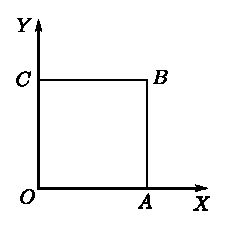
\includegraphics{vol22-figures/fig22-3.eps}}
  \end{figure}
  \begin{multline*}
  \int\limits_o^1 \int\limits_o^1 \big\{ k_1 (\xi,\eta)
  \frac{\partial^2}{\partial \xi \partial \eta} H(\xi,\eta)- H(\xi, \eta)
  \frac{\partial^2}{\partial \xi \partial \eta} k_1 (\xi,\eta)\big\} ~
  d ~ \xi ~ d ~ \eta\\ 
   = \int_Q \Big[ H(\xi,\eta) \frac{\partial k_1}{\partial \xi} ~ d \xi +
    k_1 (\xi,\eta) \frac{\partial H}{\partial \eta} ~ d  ~ \eta 
    \Big]
  \end{multline*}
  where $Q_\uparrow$ denotes the perimeter of the square $0 \le x \le 1, 0 \le
  y \le 1$ in the sense $OABC$. The integral over the vertical sides
  $AB,CD$ will be denoted by $\int_\uparrow$ and it equals 
  \begin{align*}
    \int_\uparrow ~ k_1 (\xi, \eta) \frac{\partial H}{\partial
      \eta} ~ d \eta &= \int_\uparrow ~ k_1 ~dH_1
     = \int_\uparrow ~ d(k_1H) - \int_\uparrow Hdk_1\\
    & = -\int_\uparrow ~ H ~ \frac{\partial k_1}{\partial \eta} ~ d
    \eta + (k_1 H)_{(1,1)} - (k_1H)_{(1,0)}\\ 
    & \hspace{3cm} - (k_1 H)_{(0,1)} + (k_1 H)_{(0,0)} 
  \end{align*}
\end{proposition}

Finally\pageoriginale 
\begin{multline*}
M_1 (\lambda,\mu)  = a_1 + b_1 e^\lambda + c_1 e^\mu + d_1
e^{\lambda + \mu}\\ 
   + \frac{1}{\lambda \mu} \Big[ k_1 (1,1) e^{\lambda + \mu} - k_1
    (1,0) e^{\lambda} - k_1 (0,1) e^\mu + k_1 (0,0)\\ 
     \int_{Q_\uparrow} e^{\lambda \xi + \mu \eta} \left[\frac{\partial
        k_1}{\partial \xi} d \xi - \frac{\partial k_1}{\partial \eta}
      d\eta \right] + \int\limits_o^1 \int\limits_o^1 e^{\lambda \xi +
      \mu \eta} \frac{\partial^ k_1}{\partial \xi \partial \eta} d ~
    \xi ~ d ~ \eta 
\end{multline*}
and we have a similar expression for $M_2 (\lambda, \mu)$ i.e.
\begin{align*}
   M_1 (\lambda,\mu) &= a_1 + b_1 e^\lambda + c_1 e^\mu + d_1
  e^{\lambda + \mu} + \frac{\bar{M}_1 (\lambda,\mu)}{\lambda \mu}\\ 
  M_2 (\lambda,\mu) &= a_2 + b_2 e^\lambda + c_2 e^\mu + d_2 e^{\lambda
    + \mu} + \frac{\bar{M}_2 (\lambda \mu)}{\lambda\mu} 
\end{align*}
where the functions $\bar{M}_1 (\lambda, \mu)$ and $\bar{M}_2
(\lambda, \mu)$ are entire functions of exponential type which remains
bounded when $(\lambda,\mu)$ lie in a vertical band of $C^2$ so that
$| \dfrac{M_1 (\lambda,\mu)}{\lambda \mu}| \rightarrow 0$. as
$\lambda, \mu \rightarrow \infty$ in a vertical band and in particular
when $(\lambda, \mu) \in (\sigma)$ by proposition
\ref{part2:chap3:sec8:prop1}. Thus the 
spectrum $(\sigma)$ is asymptotic\pageoriginale with the solutions of  
\begin{align*}
  & \phi_1 (\lambda, \mu) = a_1 + b_1 e^\lambda + c_1 e^\mu + d_1
  e^{\lambda + \mu } = 0\\ 
  & \phi_2(\lambda,\mu) = a_2 + b_2 e^\lambda + c_2 e^\mu + d_2
  e^{\lambda, \mu} = 0 
\end{align*}

Setting $e^\lambda = X$ and $e^\mu = Y$ we obtain
(\ref{part2:chap3:sec8:eqH1}) and (\ref{part2:chap3:sec8:eqH2}) 
and the required result follows. 

\begin{coro*}% corollary
  $|D(\lambda,\mu)|, D(\lambda,\mu)$ being the Jacobian of
  $M_1(\lambda,\mu), M_2 (\lambda,\mu)$ possesses a positive lower
  bound on $(\sigma)$. $D(\lambda,\mu)$ it asymptotic with the
  Jacobian of $\phi_1 (\lambda,\mu)$ and $\phi_2(\lambda,\mu)$ which
  is  
\end{coro*}

\begin{equation*}
  \frac{\partial^2(1_1, \varphi_2)}{(\lambda,\mu)} = \begin{vmatrix}
    b_1 e^\lambda + d_1 e^{\lambda + \mu} \quad c_1 e^\mu + d_1
    e^{\lambda + \mu}\\  b_2 e^\lambda + d_2 e^{\lambda + \mu} \quad
    c_2 e^{\mu} + d_2 e^{\lambda + \mu}  \end{vmatrix} 
\end{equation*}

When $(\lambda,\mu) \in (\sigma), (e^\lambda, e^\mu) = (\xi_i,
\eta_i)\, 
i = 1,2, (\xi_i,\eta_i)$ being the common points of $(H_1)$ and
$(H_2)$. Then 
$$
\Big[\frac{ \partial (\varphi_1,\phi_2)}{\partial
    (\lambda,\mu)}\Big]_{(\lambda,\mu) \in (\sigma)} = \xi_i ~ \eta_i
\Big[ (b_1 c_2 - b_2 c_1) + (b_1 d_2 - b_2 d_1) \xi_i + (d_1 c_2  -
  d_2 c_1) \eta_i\Big] 
$$
for $i = 1,2$.

But\pageoriginale the expression in the square bracket is precisely
the Jacobian of 
(\ref{part2:chap3:sec8:eqH1}) and (\ref{part2:chap3:sec8:eqH2}) at the
common point $(x_i,\eta_i)$ which is 
distinct from zero since the two hyperbolas do not touch each
other. In view of the conditions of proposition \ref{part2:chap3:sec8:prop1} and the remarks
following the proposition $\xi_i \eta_i \neq 0$. Thus $|
D(\lambda,\mu) |$ for $(\lambda,\mu) \in (\sigma)$ is asymptotic with
two nonzero values. Further by the usual hypothesis that the spectrum
$(\sigma)$ is `simple' i.e. $D(\lambda,\mu) \neq  0$ for any
$(\lambda, \mu) \in (\sigma)$ it follows that $| D (\lambda,\mu) |$
possesses a positive (strictly) lower bound. 

Let $A_1$ and $A_2$ be Fourier- Laplace transforms of two densities
$U_1$ and $U_2$ with supports in the square $0 \le x \le 1, 0 \le y
\le 1$ 
\begin{align*}
  U_1 * F & = \iint U_1 (\xi,\eta) F(x + \xi, y+ \eta) d ~ \xi ~ d\eta\\
  U_2 * F & = \iint U_2 (\xi,\eta) F(x+ \xi, y+ \eta) d\xi ~ d\eta
\end{align*}

We wish to prove the following
\begin{theorem*}% theorem
  The formula
  $$
  \frac{J(A,M)}{J(\lambda,\alpha)} = \sum_{\substack{\beta \neq
      \alpha\\ \beta \in (\sigma)}} \frac{[\lambda-\alpha]}{D(\beta)
    [\lambda -\beta] [\beta - \alpha] } \frac {J (M,M)} {J (\lambda,
    \beta)} \frac{J(A,M)} {J (\beta, \alpha)}+ \mathscr{R} 
  $$
  holds if $M_1$ and $M_2$ are Fourier- Laplace transforms of
  distributions $T_1$ and $T_2$  given by 
  \begin{multline*}
  T_i *F= a_i F(x,y)+ b_i F(x+ 1,y) + c_i F(x,y+1)\\
  +d_i F (x+1, y+1) +\iint k_i (\xi,\eta) F (x + \xi, y + \eta) d \xi
  \eta ~i = 1,2   
  \end{multline*}
  (provided\pageoriginale the functions $k_i (\xi,\eta)$ and the coefficients $a_i,
  b_i, c_i, d_i, i = 1,2$, satisfy the required conditions in order
  that the spectrum $(\sigma)$ should have the desirable properties;
  cf. propositions proved above). 
\end{theorem*}

If $T_1, T_2, U_1,U_2$ be replaced by $T_1(\eta), T^{(n)}_2,
U^{(n)}_1,U^{(n)}_2$ respectively where 
\begin{align*}
  T^n_i * F & = a_i F(x,y) + b_i F(x + 1,y) + c_i F(x,y + 1) + d_i F(x +
  1, y+1)\\ 
  &\quad  + \sum_{p,q=0}^{n-1} \frac{1}{n^2} k_i \left(\frac{p}{n},
  \frac{q}{n}\right )
  F\left(x + \frac{p}{n}, y + \frac{q}{n}\right), i= 1,2; \quad \text{ and }\\ 
  U^n_i * F &= \sum_{p,q = 0}^{n-1} \frac{1}{n^2} U_1 \left(\frac{p}{n},
  \frac{q}{n}\right) F \left( x +\frac{p}{n}, y + \frac{q}{n}\right), 
\end{align*}
then we know that the theorem holds for $M^n_1, M^n_2, A^n_1, A^n_2$
(with the obvious notation: $\mathscr{F} \mathscr{L} T^n_1 = M^n_1
\cdots $ etc). Hence the first step in the proof is to study the
spectrum $(\sigma^n)$ of $T^n_1$ and $T^n_2$ and its relation to
$(\sigma)$ as $n \rightarrow \infty$. 

\begin{proposition}\label{part2:chap3:sec8:prop3}% proposition 3
  $(\sigma^n)$ is contained in a vertical band which is independent of $n$.
\end{proposition}

The\pageoriginale proof of the proposition is analogous to that of
Proposition \ref{part2:chap3:sec8:prop1} 
and we shall give only a partial verification. For instance we prove
that if $(\lambda,\mu) \in (\sigma^n)$ and $\lambda = \lambda_o + i
\lambda, \mu = \mu_o + i ~ \mu_1$, then i) $\lambda_o, \mu_o$ cannot
both tend to $+ \infty$; ii) $\lambda_o$ cannot tend to $+ \infty$
when $\mu_o \rightarrow - \infty$, iii) when $| \lambda_o | < m<
\infty$, then $\mu_o$ cannot tend to $+ \infty$. 

i)~ For $(\lambda,\mu) \in (\sigma^n)$, we have $M^n_i (\lambda,\mu)
  = 0, i= 1,2$. If $\lambda_o \rightarrow + \infty, \mu_o \rightarrow
  \infty$, we write 
$$
\displaylines{\hfill 
     - d_1 = a_1 e^{-\lambda - \mu }+ b_1 e^{-\mu} + c_1 e^{-\lambda}
    + e^{-\lambda - \mu} \sum \frac{1}{n^2} k_1 \left(\frac{p}{n},
    \frac{q}{n}\right) \exp \frac{\lambda p + \mu q} {n}\hfill \cr
    \hfill | d_1 |  \le | a_1 | e^{- \lambda_o - \mu_o} + | b_1 |
    e^{-\lambda_o} + | c_1 | e^{- \lambda_o} + e^{- \lambda_o - \mu_o}
    ~L_1 \int\limits_o^1 \int\limits_o^1 ~ e^{\lambda_o \xi + \mu_o
      \eta} ~ d \xi d \eta \hfill \cr
    \text{where}\hfill 
    L_1 = \sup_{\substack{0 \le \xi \le 1 \\ 0 \le \eta \le 1}} ~ k_1
    (\xi,\eta)\hfill }
  $$
  since $(x,y) \rightarrow e^{\lambda_o x + \mu_o y}$ is an increasing
  function of $(x,y)$ when $\lambda_o,\mu_o > 0$ which may be assumed
  to be the case since $\lambda_o, \mu_o$ both tend to $+ \infty$. 

  Or 
  \begin{gather*}
    | d_1 | \le | a_1 | e^{-\lambda_o - \mu_o } + | b_1 | e^{- \mu_o}
    | c_1 | e^{-\lambda_o}+ e^{- \lambda_o - \mu} L_1
    \frac{(e^{\lambda_o -1})(e^{\mu_o -1})}{\lambda_o \mu_ o}\\
    \rightarrow 0 \text{ as } \lambda_o,  \mu_o \rightarrow + \infty.
  \end{gather*}
  
  This\pageoriginale contradicts the hypothesis that $d_1 \neq 0$.

ii)~ If $\lambda_o \rightarrow + \infty, \mu_o \rightarrow - \infty$, we write
  \begin{gather*}
    - b_1 = a_1 e^{-\lambda} + c_1 e^{\mu - \lambda} + d_1 e^{\mu} +
    e^{-\lambda} \sum_p \sum_q \frac{1}{n^2} k_1 (\frac{p}{n},
    \frac{q}{n}) \exp \frac{\lambda p + \mu q }{n} \\
    | b_1 | \le | a_1 | e^{- \lambda_o} +  | c_1 | e^{\mu_o - \lambda_o}
    + | d_1 | e^{\mu_o} + e^{-\lambda_o} \sum_{p=0}^{n-1} \sum_{q =
      0}^{n-1} \frac{1}{n^2} | k_1 (\frac{p}{n}, \frac{q}{n}) | \exp
    \frac{\lambda_o p}{n} 
  \end{gather*}
  since $\exp \frac{\mu_o q}{n} \le 1$
$$
\displaylines{ 
  \text{i.e.,}\hfill | b_1 | \le | a_1 | e^{-\lambda_o} + | c_1 | e^{\mu_o -
  \lambda_o} + | d_1 | e^{\mu_o} + e^{-\lambda_o} L_1 \int\limits_o^1
  \int\limits_o^1 e^{\lambda_o \xi} ~ d \eta d \xi\hfill \cr 
  \hfill = | a_1 | e^{- \lambda_o} + | c_1 | e^{\mu_o - \lambda_o} + | d_1 |
  e^{\mu_o} + e^{-\lambda_o} L_1 \frac{e^{\lambda_o} -1}{\lambda_o}
  \hfill }
  $$
  $\rightarrow 0$ as $\lambda_o \rightarrow + \infty$ and $\mu_o
  \rightarrow - \infty$ which is not possible since $b_1 \neq 0$. 

iii)~ Suppose that $| \lambda_o | < m_1$ and $\mu_o \rightarrow +
  \infty$. We write 
  \begin{align*}
    0 & = a_1 e^{- \mu } + b_1 e^{\lambda - \mu} + c_1 + d_1 e^{-
      \mu}+ e^{-\mu}
    \sum_{p = 0}^{n-1} \sum_{q=0}^{n-1} k_1 \left(\frac{p}{n},\frac{q}{n}\right)
    \exp \frac{\lambda p + \mu q}{n}\\ 
    0 & = a_2 e^{- \mu } + b_2 e^{\lambda - \mu} + c_2 + d_2 e^{- \mu}
    + e^{-\mu}
    \sum_{p = 0}^{n-1} \sum_{q=0}^{n-1} k_2 \left(\frac{p}{n},\frac{q}{n}\right)
    \exp \frac{\lambda p + \mu q}{n} 
  \end{align*}

Eliminating\pageoriginale $e^\lambda$ from these we get
\begin{multline*}
  | c_1 d_2 - c_2 d_1 | \le | a_1 d_2 - a_2 d_1 | e^{- \mu_o} + | b_1
  d_2 - b_2 d_1 | \\
  e^{\lambda_o - \mu_o} + e^{-\mu_o} L_2 \int\limits_o^1
  \int\limits_o^1 e^{\mu_o \eta} d\xi d \eta 
\end{multline*}
where $L_2$ depends upon the supremum of $| d_1 k_2 (x,y) - d_2 k_1
(x,y) | e^{\lambda_o x}$ for $0 \le x \le 1, 0 \le y \le 1$. i.e. the
last term is majorised by $e^{-\mu_o} ~ L_2 \dfrac{(e^{\mu_o}
  -1)}{\mu_o}$. Hence right hand side of the above inequality
$\rightarrow 0$ when $| \lambda_o | < m$ and $\mu_o \rightarrow +
\infty$. But this contradicts the assumption that $c_1 d_2 - c_2 d_1
\neq 0$. 

\heading{Summation of the series} $S_n (\lambda,\alpha_n)$.

$$
S_n (\lambda, \alpha_n) = \sum_{\beta^n \in (\sigma^n)} \frac{[\lambda
    - \alpha^n]}{D(\beta^n)[\lambda - \beta^n][\beta^n - \alpha^n]}
\frac{J(M^n,M^n)}{J(\lambda,\beta^n)}
\frac{J(A^n,M^n)}{J(\beta^n,\alpha^n)} + \mathscr{R}^n 
$$
(where $\mathscr{R}^n$ can be got from $\mathscr{R}$ by replacing
$M,A$ by $M^n,A^n$ respectively), where $\lambda = (\lambda_1,
\lambda_2)$ denotes a point in $C^2$. The functions \break $M^n_1 (\lambda),
M^n_2(\lambda),A^n_1(\lambda), A^n_2(\lambda)$ are periodic in
$\lambda_1,\lambda_2$ with periods $2 \pi ni$. The same statement
holds for the Jacobian $D_n(\lambda)$ of the functions $M^n(\lambda)$
as also the two determinants of Jacobi: 
$$
\frac{J(M^n,M^n)}{J(\lambda,\alpha)} \text{ and }
\frac{J(A^n,M^n)}{J(\beta,\alpha)} 
$$
considered\pageoriginale as functions of couples of points of $C^2, (\lambda,
\alpha)$ and $(\beta,\alpha)$, $\lambda, \alpha, \beta \in C^2$. These
are therefore periodic functions of the four complex variables with
the same period $2n \pi i$. Moreover $M^n_1$, and $M^n_2$ are
polynomials in $\exp \dfrac{\lambda_1}{n}, \exp \dfrac{\lambda_2}{n}$
so that the zeros $\beta_n$ in the spectrum $(\sigma^n)$ can be
arranged in $2n^2$ classes, each of these classes being situated in a
plane parallel to the purely imaginary plane of $C^2$ and forming in
this plane a network of squares of sides $2 \pi n$. By virtue of this
remark, the series $S_n(\lambda,\alpha^n)$, which is absolutely
convergent can be broken up in $2n^2$ partial sums corresponding to
$2n^2$ classes in which the spectrum $(\sigma^n)$ is divided. In each
of these partial sums the factors 
$$
\frac{1}{D_n(\beta^n)} \frac{J(M^n,M^n)}{J(\lambda,\beta^n)}
\frac{J(A^n,M^n)}{J(\beta^n,\alpha^n)} 
$$
has the same value for all the terms of the partial sum $(\lambda,
\alpha^n$ are fixed) due to the periodicity of the functions
$D_n,M^n_1,M^n_2, A^n_1, M^n_2$. We shall then choose a representative
$\beta^n$  in each class which will be fixed (for the class $\lambda,
\sigma^n$, we choose $\alpha^n$ itself as its representative). It is
necessary to calculate, for each class 
\begin{multline*}
  \sum_{h = - \infty}^{+ \infty} \sum_{k = - \infty}^{+ \infty}
  \frac{\lambda_1 - \alpha^n_1}{(\lambda_1- \beta^n_1 - 2nh \pi
    i)(\beta^n_1 + 2nh \pi i - \alpha^n_1)}\\ 
  \frac{\lambda_2 -
    \alpha_2^n}{(\lambda_2 - \beta_2^n - 2nk \pi i)(\beta^n_2 + 2n k \pi i
    - \alpha^n_2)} 
\end{multline*}
if\pageoriginale $\alpha^n$ does not belong to the class considered and 
$$
\sum_{h = - \infty}^{+ \infty_{'}} \sum_{k = - \infty}^{+ \infty_{'}}
\frac{\lambda_1 - \alpha^n_1}{(\lambda_1- \alpha^n_1 - 2nh' \pi i)(2nh
  \pi i)} \frac{\lambda_2 - \alpha^n_2}{(\lambda_1- \alpha^n_1 - 2nk
  \pi i)(2nk \pi i)} 
$$
if $\alpha^n$ belongs to the class considered. $(\sum' \sum'$ denotes
that that value $h= 0, k= 0$ is excluded in the summation). The
calculation of these two sums is classical and gives  
$$
\frac{1}{n^2} \left[\frac{1}{\exp \left(\frac{\lambda_1 -
      \beta^n_1}{n}\right)-1} 
  - \frac{1}{\exp \frac{\alpha^n_1 - \beta^n_1}{n}-1}\right] \left[
  \frac{1}{\exp \left(\frac{\lambda_2 - \beta^n_2}{n}\right) -1} - \frac{1}{\exp
    \frac{\alpha^n_2 - \beta^n_2}{n} -1}\right] 
$$
in the first case and  
$$
\frac{1}{n^2} \left[ \frac{1}{\exp \left(\frac{\lambda_1 - \beta^n_1}{n}\right)
    -1} - \frac{n}{\lambda_1 - \alpha^n_1} + \frac{1}{2}\right] \left[
  \frac{1}{\exp\frac{\lambda_2 - \alpha^n_{2}}{n}-1} -
  \frac{n}{\lambda_2 - \alpha^n_2} + \frac{1}{2} \right] 
$$
is the second.

As $\dfrac{J(A^n,M^n)}{J(\lambda^n,\alpha^n)} = 0$ since $\alpha^n \in
e (\sigma^n)$, we see that the series $S_n(\lambda, \alpha^n)$ can now
be put in the form of a finite sum (with $2n^2 -1$ terms) each of
these terms corresponding to classes in which the spectrum
$(\sigma^n)$ is divided. Denoting the classes by capital letters, 
$$
a_n = \text{ class  of } \alpha^n, \mathscr{B}_n = \text{ class of } \beta^n,
$$
the\pageoriginale representatives $\alpha^n,\beta^n$ being fixed in their class, we
can write 
\begin{multline*}
S_n(\lambda,\alpha^n) = \frac{1}{n_2} \sum_{\mathscr{B}^n \neq a^n}
\left[ \frac{1}{\exp \left(\frac{\lambda_1 - \beta^n_1}{n}\right) -1}
  -\frac{1}{\exp\left(\frac{\alpha^n_1 - \beta^n_1}{n}\right)-1}\right]\\ 
  \hspace{1.7cm}\left[ \frac{1}{\exp\left(\frac{\lambda_2 -
        \beta^n_2}{n}\right)-1}
    -\frac{1}{\exp \left(\frac{\alpha^n_2 -
        \beta^n_2}{n}\right)-1}\right]\\ 
  \frac{1}{D_n(\beta^n)} ~ \frac{ J(M^n,M^n)}{J(\lambda,\beta^n )}
  ~\frac{J(A^n,M^n)}{J(\beta^n, \alpha^n)} \tag{1}
\end{multline*}

\heading{Behaviour of $S_n(\lambda,\alpha^n)$ for $n$ large.}

Applying Taylor's formula for the function $\dfrac{z}{e^z -1}$ which
is holomorphic in the neighbourhood of the origin, we have 
$$
\frac{x}{e^x -1} = 1 - \frac{x}{2} + \frac{x^2}{2 \pi i} \int_0
\frac{dz}{z(z-x)(e^z -1)} 
$$
where $C$ is the circumference of a circle with centre origin and
radius $< 2 \pi $ ($2 \pi$ is the radius of convergence of the
Taylor's series of the function about the origin). Let $x =
\dfrac{\lambda}{n}$ with $| \lambda | < \pi n$ so that $| x | <
\pi$. Dividing by $\lambda$, we have 
$$
\frac{1}{n(e^{1/n}-1)} - \frac{ 1}{\lambda} + \frac{1}{2 \pi} =
\frac{\lambda}{2 \pi ~ i ~ n^2} \int\limits_C
~\frac{dz}{z(z-\frac{\lambda}{n})(e^z -1)}, \lambda \neq 0 
$$
similarly\pageoriginale for $| \mu | < \pi ~ n$,
$$
\frac{1}{n(e^{\mu/n}-1)} - \frac{1}{\mu} + \frac{1}{2n} = \frac{\mu}{2
  \pi ~ i ~n^2} \int\limits_C \frac{dz}{z(z- \frac{\mu}{n}) (e^z -1)},
\mu \neq 0 
$$
subtracting, 
\begin{multline*}
  \frac{1}{n(e^{\lambda/n}-1)} - \frac{1}{n(e^{\mu/n}-1)} -
  \left(\frac{1}{\lambda} - \frac{1}{\mu}\right) = \frac{1}{2 \pi  i n}
  \int\limits_C \Bigg[ \frac{\frac{\lambda}{n}}{z - \frac{\lambda}{n}}
    -\frac{ \frac{\mu}{n}} {z - \frac{\lambda}{n}} \Bigg]\\
  \frac{dz}{z(e^z -1)} = \frac{\lambda - \mu}{ 2 \pi in^2} \int\limits_C
  \frac{dz}{\left(z - \frac{\lambda}{n}\right)\left(z -
    \frac{\mu}{n}\right)(e^z -1)}  
\end{multline*}

The length of $C$ is $< 4 \pi^2, | \dfrac{\lambda}{n} | < \pi$ and $|
\dfrac{\mu}{n} | < \pi$. Hence $| z - \dfrac{\lambda}{n}| \ge \pi, | z
- \dfrac{\mu}{n} | \ge \pi$; let $M$ denote $\underset{|z|=R}{\max} ~
| \dfrac{1}{e^z -1}|, (R < 2 \pi)$. Then 
$$
\Big| \frac{1}{n(e^{\lambda/n}-1)} - \frac{1}{n(e^{\mu/n}-1)} -
\left(\frac{1}{\lambda} - \frac{1}{\mu}\right) \Big| \le C_o  ~
\frac{| \lambda -\mu |}{n^2} 
$$
with $C_o = \dfrac{2M}{\pi}$ and $| \lambda | < \pi n, | \mu |\le \pi
n$. Changing $\lambda$ into $\lambda_1 - \beta^n_1,\mu$ into
$\alpha^n_1 - \beta^n_1$ or $\lambda$ into $\lambda_2 - \beta^n_2,
\mu$ into $\alpha^n_2 - \beta^n_2$, we have the majorisation 
\begin{align*}
   \Bigg| \frac{1}{n} \left[ \frac{1}{\exp \left(\frac{\lambda_1 -
        \beta^n_1}{n}\right) -1} -  \frac{1}{\exp \left(\frac{\alpha^n_1 -
        \beta^n_1}{n}\right) -1}  \right] & - \frac{\lambda_1 -
    \alpha^n_1}{(\lambda_1 - \beta^n_1 ) (\beta^n_1 - \alpha^n_1 )}\Bigg|\\
  & \hspace{2cm}\leq \frac{c_0}{n^2} | \lambda_1 - \alpha^n_1 | \\ 
   \Bigg| \frac{1}{n} \left[ \frac{1}{\exp \left(\frac{\lambda_2 -
        \beta^n_2}{n}\right) -1} -  \frac{1}{\exp \left(\frac{\alpha^n_2 -
        \beta^n_2}{n}\right) -1}  \right] & - \frac{\lambda_2 -
    \alpha^n_2}{(\lambda_2 - \beta^n_2 ) (\beta^n_2 - \alpha^n_2 )} \Bigg|\\
  & \hspace{2cm} \leq \frac{c_0}{n^2} | \lambda_2 - \alpha^n_2 | 
\end{align*}
provided\pageoriginale that
\begin{equation}
  \left.
  \begin{aligned}
    & | \lambda_1 - \beta^n_1| \leq \pi_n,  |\lambda_2 - \beta^n_2 |
    \leq \pi n \\ 
    & |\beta_1 - \alpha^n_1 | \leq \pi_n,  |\beta^n_2 - \alpha^n_2 | \leq \pi n 
  \end{aligned} \tag{2}\label{part2:chap3:sec8:eq2}
  \right \} 
\end{equation}
[ Note that $|\lambda_1 - \alpha_1|$ and $|\lambda_2 - \alpha_2|$ are
  independent of $\rho_1, \beta_2$ and therefore fixed in the
  summation (\ref{part2:chap3:sec1:eq1}) ]. 

Using the majorisation (\ref{part2:chap3:sec8:eq2}), we shall study
(\ref{part2:chap3:sec1:eq1}) and compare it with
a finite sum 
\begin{multline*}
  \tau (\lambda,  \alpha ) = \frac{1}{n^2} \sum_{\beta \neq \alpha}
  \left[ \frac{1}{\exp \left(\frac{\lambda_1 - \beta_1}{n}\right) -1} -
    \frac{1}{\exp \left(\frac{\alpha_1 - \beta_1}{n}\right) -1} \right] \\ 
  \left[ \frac{1}{\exp \left(\frac{\lambda_2 - \beta_2}{n}\right) -1} -
    \frac{1}{\exp \left(\frac{\lambda_2 - \rho_2}{n}\right) -1} \right]
  \frac{1}{D(\beta )} \frac{J(M, M)}{J (\lambda, \beta )} \frac{J(A,
    M)}{J(\beta,  \alpha )}. 
\end{multline*}

The\pageoriginale summation in $\beta$ is made for $\beta \in (\sigma )$ which are
``near'' to those $\beta^n$ which are the chosen representatives of the
$2n^2 - 1$ classes $\mathscr{B}_n \neq a_n$. It is necessary for this
to compare the functions $M$ and $M^n, A$ and $A^n, (\sigma)$ and
$(\sigma^n)$. 

\heading{Comparison of $M$ with $M^n$ and of $A$ with $A^n$.}

\begin{equation}
  \left.
  \begin{aligned}
    M_1(\lambda ) & =  a_1 + b_1 e^{\lambda_1} + c_1 e^{\lambda_2} +
    d_1 e^{\lambda_1 + \lambda_2} + N_1 (\lambda ) \\ 
    M_2(\lambda ) & = a_2 + b_2 e^{\lambda_1} + c_2 e^{\lambda_2} +
    d_2 e^{\lambda_1 + \lambda_2} + N_2 (\lambda ) 
  \end{aligned} \tag{3}\label{part2:chap3:sec8:eq3}
  \right \}\\ 
\end{equation}
\begin{equation}
  \left.
  \begin{aligned}
    M^n_1(\lambda ) & =  a_1 + b_1 e^{\lambda_1} + c_1 e^{\lambda_2} +
    d_1 e^{\lambda_1 + \lambda_2} + N^n_1 (\lambda ) \\ 
    M^n_2 (\lambda ) & = a_2 + b_2 e^{\lambda_1} + c_2 e^{\lambda_2} +
    d_2 e^{\lambda_1 + \lambda_2} + N^n_2 (\lambda ) 
  \end{aligned} \tag{4}\label{part2:chap3:sec8:eq4}
  \right \} 
\end{equation}
 
 Hence it is sufficient to compare $N$ and $N^n$. The calculation will
 be similar for $A$ and $A^n$. 

We shall now suppose (for simplifying the proof) that the functions
$k_1,  k_2,  a_1, a_2$ in $R^2$ are\pageoriginale indefinitely differentiable with
compact support contained in the square $0 \leq x_1 \leq 1, 0 \leq x_2
\leq 1$. Then the functions $A(\lambda ), N(\lambda )$ decrease rapidly
when $\lambda$ recedes to infinity keeping itself in a vertical
plane. Hence the functions such as 
$$
\frac{1}{n^2} k_1 \left(\frac{y_1}{n},  \frac{y_2}{n}\right) \exp
\left(\frac{\lambda_1 y_1 + \lambda_2 y_2}{n}\right) = K^n_1 (y_1,  y_2) 
$$
are indefinitely differentiable with compact support contained in the
square $0 \leq y_1 \leq n, 0 \leq y_2 \leq n$ and we can write for
example 
$$
N^n_1 (\lambda ) = \sum_{p, q} K^n_1 (p, q)
$$
where the summation is made over all the couples of integers $(p,
q)$. In order to evaluate this sum it suffices to apply Poisson's
formula. The Fourier transform of $K^n_1 (y_1, y_2)$ is ($\mu_1,
\mu_2$ being real): 
{\fontsize{10}{12}\selectfont
\begin{align*}
\mathscr{F} [K^n_1] &= \iint K^n_1 (y_1, y_2) \exp [-2 \pi i (\mu_1 +
  \mu_2 y_2)] dy_1 ~ dy_2  \\
  & = \frac{1}{n^2} \iint  K_1 (y_1, y_2) \exp [\left(\frac{\lambda_1}{n} -
    2 \pi \mu_1 \right) y_1 + \left(\frac{\lambda_2}{n} - 2 \pi i
    \mu_2 \right) y_2] dy_1 dy_2 \\ 
  & = \iint k_1 (u)\exp \langle \lambda - 2 \pi i \mu n, u \rangle du
  = N_1 (\lambda - 2 \pi i \mu n) 
\end{align*}}\relax
Hence by Poisson's formula,
\begin{equation}
  \left.
  \begin{aligned}
    N^n(\lambda ) & = \sum^{~}_{h, k}N(\lambda_1 - 2 \pi ihn,  \lambda_2 -
    2 \pi ikn) \\ 
    A^n(\lambda ) & = \sum_{h, k} A (\lambda_1 - 2 \pi ihn,  \lambda_2
    - 2 \pi ikn) 
  \end{aligned} \tag{5}\label{part2:chap3:sec8:eq5}
  \right\} 
\end{equation}
\begin{equation*}
  \left.
  \begin{aligned}
    N^n(\lambda ) - N(\lambda ) & = \sum'_{h, k}N (\lambda_1 - 2 \pi
    ihn, \lambda_2 - 2 \pi ikn) = M^n(\lambda ) - M(\lambda ) \\ 
    A^n(\lambda ) - A (\lambda ) & = \sum'_{h, k} A (\lambda_1 - 2 \pi
    ihn, \lambda_2 - 2 \pi ikn)  
  \end{aligned} \tag{6}\label{part2:chap3:sec8:eq6}
  \right\}
\end{equation*}
where\pageoriginale the accent indicates that in the summation the couple $h=0, ~
k=0$ is excluded. 

\heading{Majorisation of the difference $N^n -N$ and $A^n - A$.}

As $N$ decreases rapidly in the vertical bound, we have	
$$
|N (\lambda_1, \lambda_2 ) | \leq \frac{c_1 (r)}{|\lambda_1 \lambda_2 |^r}
$$
in a vertical band where $r$ is a positive integer, arbitrarily large
and where $c_1(r)$ is a constant which depends on $r$ and the function
$k_1(x_1, x_2)$. Hence 
$$
|M^n_1 (\lambda ) - M_1 (\lambda ) | \leq c_1 (r) \sum'_{h, k}
\frac{1}{| \lambda_1 - 2 \pi inh |^r |\lambda_2 - 2 \pi ink |^r}  
$$
(for $\lambda_1$ and $\lambda_2$ different from the multiples of $2
\pi in$; this restriction is artificial). 

Majorising the second member for $r \geq 3$, it is easy to verify that 
\begin{equation}
  |M^n_1(\lambda ) - M_1(\lambda ) | \leq \frac{c_2(r)}{(2 \pi n)^r}
  \tag{7}\label{part2:chap3:sec8:eq7} 
\end{equation}
if
\begin{equation}
  |Im \lambda_1 |\leq \pi n, | Im \lambda_2 | \leq \pi n
  \tag{8}\label{part2:chap3:sec8:eq8} 
\end{equation}
and we have analogous inequalities for the functions $M_2, A_1, A_2$
under\pageoriginale the same conditions (\ref{part2:chap3:sec8:eq8}). We can always denote by $c_2(r)$ the
positive constant figuring in the numerator of the second member of
(\ref{part2:chap3:sec1:eq1}) by taking the same constant for the functions. 

\heading{The volume $V_n$; zeros of $M(\lambda )$ in the interior of $V_n$.}

We know that $(\sigma)$ and $(\sigma^n)$ are in a fixed vertical band
$\mathscr{B}$ independent of $n$. We shall intersect the vertical band
by a horizontal band in $C^2$ defined by (\ref{part2:chap3:sec8:eq8}). Its section by a
vertical plane is a square of side $2 \pi n$. Such a square contains
one and only one point of each of the $2n^2$ classes in which
$(\sigma^n)$ is decomposed, since each of these $2n^2$ classes form,
in its plane, which is vertical, a network of squares of side $2 \pi
n$. It follows that the volume $V_n $ in $C^2$ contains exactly $2n^2$
points of the spectrum $(\sigma^n)$. We wish to find the points of
$(\sigma )$ which are also in $V_n$. We first recall a classical
result due to Kronecker. 

Let $f, g, h$ be three functions continuously differentiable in a
region in $R^3$. Let $V$ be a volume contained in the region with
boundary $S$. Then 
$$
\displaylines{\hfill
  m = - \frac{1}{4 \pi} \iint_S ( A \cos \lambda + B \cos \mu + C \cos
  \nu) dS\hfill \cr 
  \text{where}\hfill
  A = \left[ f \frac{D(g, h)}{D(y, z)} + g \frac{D(h, f)}{D(y, z)} + h
    \frac{D(f, g)}{D(y, z)}\right] \frac{1}{[f^2 + g^2 + h^2]^{3/2}}
  \hfill }
$$
$B, C$\pageoriginale being analogously defined and cos $\lambda, \cos \mu,  \cos,
\gamma$ are the direction cosines of the interior normal to $S$ and
$m$ equals the difference between the number of solutions lying in $V$
of the systems $f = g = h = 0$ for which $\dfrac{D(f, g, h)}{D(x, y,
  z)} > 0$ and the number of solutions for which $\dfrac{D(f, g,
  h)}{D(x, y, z)} < 0$. We shall use the analogue of this proposition
in $R^4 = C^2$ i.e., 

If $f_1,  f_2,  f_3, f_4$ are four functions which are $(C, 1)$ in a
region of $R^4$, then  
$$
\displaylines{\hfill 
  \qquad m = - \frac{1}{2 \pi^2} \iiint (A_1 \cos \lambda_1 + A_2 \cos
  \lambda_2 + A_3 + A_4 \cos \lambda_4) dS \hfill \cr
  \text{with}\hspace{.7cm}
  A_1 = \left[ \sum_{f_1} \frac{D(f_2, f_3, f_4)}{D(x_2, x_3, x_4)}
    \right] \frac{1}{\left[\sum\limits^4_{1=1}f_i^2\right]^2} \hfill }
$$
and $A_2,  A_3, A_4$ similarly defined, where $m$ is defined as above
for the system of equations $f_1 = f_2 = f_3 = f_4 = 0$ and the
Jacobian $\frac{D(f_1, f_2, f_3, f_4)}{D(x_1, x_2, x_3, x_4)} $. The
integral on the right hand side will be called the Kronecker
integral. 

We consider the following analytic transformation of $C^2$ into itself,
$$
(\lambda_1,  \lambda_2 ) \rightarrow (M_1(\lambda_1,  \lambda_2), M_2
(\lambda_1,  \lambda_2)) 
$$
This can be considered as a transformation of $R^4$ into
itself. Instead\pageoriginale of the four variables which are the real and imaginary
parts of both $\lambda_1, \lambda_2$, we take $\lambda_1,
\bar{\lambda_1}, \lambda_2,  \bar{\lambda_2}$. Then  
\begin{align*}
  dM_1 = \frac{\partial M_1}{\partial \lambda_1} d\lambda_1 +
  \frac{\partial M_1}{\partial \lambda_2} d\lambda_2 \text{ and } \\ 
  dM_2 = \frac{\partial M_2}{\partial \lambda_1} d\lambda_1 +
  \frac{\partial M_2}{\partial \lambda_2} d\lambda_2,  
\end{align*}
as $M_1, M_2$ are analytic. The volume elements which correspond to
each other by this transformation are proportional to  
$$
d \lambda_1 \wedge d \bar{\lambda_1} \wedge d \lambda_2 \wedge d
\bar{\lambda_2} \text{ and } dM_1 \wedge d\bar{M_1} \wedge dM_2 \wedge
d\bar{M_2} 
$$
Now
\begin{align*}
  d\bar{M}_1 & = \frac{\partial \bar{M}_1}{\partial \lambda_1} d
  \bar{\lambda_1} + \frac{\partial \bar{M}_1}{\partial \lambda_2} d
  \bar{\lambda}_2 \text{ and } \\ 
  d\bar{M}_2 & = \frac{\partial \bar{M}_2}{\partial \lambda_1} d
  \bar{\lambda_1} + \frac{\partial \bar{M}_2}{\partial \lambda_2} d
  \bar{\lambda}_2 
\end{align*}
Hence 
\begin{align*}
dM_1 & \wedge d\bar{M}_1  \wedge dM_2 \wedge d \bar{M}_2 \\
  & = \left[ \frac{\partial M_1}{\partial \lambda_1}
    \frac{\overline{\partial M_1}}{\partial \lambda_1} \frac{\partial
      M_2}{\partial \lambda_2} \frac{\overline{\partial M_2}}{\partial
      \lambda_2}  - \frac{\partial M_1}{\partial \lambda_1}
    \frac{\overline{\partial M_1}}{\partial \lambda_2} \frac{\partial
      M_2}{\partial \lambda_2}  \frac{\overline{\partial
        M_2}}{\partial \lambda_1} - \frac{\partial M_1}{\partial
      \lambda_2} \frac{\overline{\partial M_1}}{\partial \lambda_1}
    \frac{\partial M_2}{\partial \lambda_1}\right.\\ 
    & \left.\hspace{2cm} \frac{\overline{\partial
        M_2}}{\partial \lambda_2}  + \frac{\partial M_1}{\partial
      \lambda_2} \frac{\overline{\partial M_1}}{\partial \lambda_2}
    \frac{\partial M_2}{\partial \lambda_1}  \frac{\overline{\partial
        M_2}}{\partial \lambda_1} \right] d \lambda_1 \wedge d
  \bar{\lambda_1} \wedge \lambda_2 \wedge d \bar{\lambda_2} \\ 
  &= \frac{D(M_1,  M_2)}{D (\lambda_1,  \lambda_2)}
  \frac{D\overline{(M_1,  M_2)}}{D (\lambda_1,  \lambda_2 )} d
  \lambda_1 \wedge d \bar{\lambda_1} \wedge d \lambda_2 \wedge d
  \bar{\lambda_2} 
\end{align*}

Thus\pageoriginale the Jacobian of the transformation under consideration is always
real and $\geq 0$. Taking real and imaginary parts of $M_1$ and $M_2$
the system $M_1 =0,  M_2 = 0$ is equivalent to the four equations $f_i
= 0 ~ i = 1, 2, 3, 4$. The Kronecker integral which can be briefly
denoted by $- \dfrac{1}{2 \pi^2}$ $\iiint K (M_1,  M_2) dS$ in this case
gives $m$ exactly equal to the number of solutions of the system $f_i
= 0$ in the volume $V$ enclosed by $S$ (since the Jacobian does not
change sign) i.e., the number of elements of $(\sigma) in V$. 

\begin{proposition}\label{part2:chap3:sec8:prop4}%proposi 4.
  The volume $V_n$ contains $2n^2$ points of $\sigma$ for $n$
  sufficiently large. 
\end{proposition}

We know that $V_n$ contains $2n^2$ points of $(\sigma^n)$. Using
Kronecker's result it follows that 
$$
2n^2 = \int_{\partial V_n} K (M^n_1,  M^n_2) dS
$$
where $\partial V_n$ denotes the boundary of $V_n$ whose measure is of
the form $c_3 n^2$, where $c_3$ is a fixed constant (viz. the product
of $4 \pi^2$ by the length of the parameter of the right section of
the vertical band $\mathscr{B}$) and the proposition will be proved if
we know that  
\begin{equation}
  2n^2 = \int_{\partial V_n} K (M_1,  M_2)d S\tag{i}\label{part2:chap3:sec8:eqi}
\end{equation}

Consider\pageoriginale the difference $K (M_1,  M_2) - K (M^n_1,  M^n_2)$ in
$\partial V_n$. Let $\lambda_1 = x_1 + ix_2,  \lambda_2 = x_3 + ix_4,
M_1 = f_1 + if_2,  M_2 = f_3 + if_4, M^n_1 = f^n_1 + if^n_2, M^n_2 =
f^n_3 + if^n_4$ where the $f'$s are real valued functions of the four
real variables $x_1,  x_2,  x_3,  x_4$. For $(\lambda_1,  \lambda_2)
\in V_n,  | M_i - M^n_i | \leq \dfrac{c_2 (r)}{(2 \pi n)^r} i = 1,
2$. Hence 
$$
|f_i - f^n_i | \leq | \frac{c_2 (r)}{(2 \pi n)^r} ~i = 1, 2, 3, 4.
$$
Similarly $| \dfrac{\partial f_i} {\partial x_j} -   \dfrac{\partial
  f^n_i} {\partial x_j}| \leq \dfrac{c'_2 (r)}{(2 \pi n)^r}$ for
$(\lambda_1,  \lambda_2) \in V_n$, since the partial derivatives of
the $f_i$ with respect to $x_j$ are exactly of the same form as the
$f_i$. 

We consider the difference $K(M_1,  M_2) - K(M^n_1, M^n_1)$ on
$\partial v_n$. In $K(M_1,  M_2)$ the $f_i$ and $\dfrac{\partial
  f_i}{\partial x_j}$ may be regarded as a finite set of variables
$u_1, u_2, \ldots $ and $K(M^n_1, M^n_2)$ is the same function with
the variables $f_i$ and $\dfrac{\partial f_i}{\partial x_j}$ replaced
by $f^n_i$ and $\dfrac{\partial f^n_i}{\partial x_j}$ respectively or
the variables $u_1,  u_2, \ldots$ replaced by $u^n_1,  u^n_2, \ldots$
respectively. Hence applying mean value theorem of differential
calculus, 
\begin{equation}
  | K(M_1,  M_2) - K(M^n_1,  M^n_2)| \leq \frac{c_3(r)}{(2 \pi n)^r} L
  \text{ on } \partial V_n \tag{ii}\label{part2:chap3:sec8:eqii} 
\end{equation}
where $L$ depends on the maximum modulus of the derivatives of $K$
with respect to $u_1, u_2, \ldots$ over a region which contains $(u_1,
u_2, \ldots)$\pageoriginale as also $(u^n_1, u^n_2, \ldots)$ while $(\lambda_1,
\lambda_2) = (x_1, x_2, x_3, x_4)$ varies in $\partial V_n$. Since
$|u_i - u^n_i| = 0 (\dfrac{1}{n^r})$ in $V_n$ and therefore on
$\partial V_n$, for $n \geq N_1$, and since $\dfrac{\partial
  K}{\partial u_i}$ are continuous functions of $(u_1, u_2, \ldots)$
in estimating $L$ it is enough to consider the maximum modulus of
$\dfrac{\partial K}{\partial u_i}$ when $(\lambda_1,  \lambda_2) \in
\partial V_n$. Now the numerator of $K(u_1, u_2, \ldots)$ is a
homogeneous polynomial in all the $u$'s of total degree $4$ with
coefficients which are functions of $\lambda_1,  \lambda_2$ with
maximum moduls $\leq 1$ and the denominator is $2 \pi^2 (u^2_1 + u^2_2
+ u^2_3 + u^2_4)$ or $2 \pi^2 [|M_1(\lambda)|^2 +
  |M_2(\lambda)|^2]$. Both the numerator and denominator as also their
partial derivatives with respect to $u_i$ are uniformly bounded on
$\partial V_n$ since they are uniformly bounded on $\mathscr{B}$ and
$V_n$ is a closed subset of $\mathscr{B}$. Hence $L$ can be found to
be a fixed positive number which does not depend on $n$ if we prove
that the denominator of $K$ i. e. $2 \pi^2 [|M_1(\lambda)|^2 +
  |M_2(\lambda ) |^2]$ is bounded below uniformly for $(\lambda_1,
\lambda_2) \in \partial V_n$ by a fixed number $ > 0$ which does not
depend on $n$. 

First we consider two vertical parts of $\partial V_n$, denoted by
$(\partial V_n)_1$ i. e. parts contained in $\partial \mathscr{B}$. On
$\partial \mathscr{B}$ real parts of $\lambda_1,  \lambda_2$ are
constant and the imaginary parts vary from $- \infty$ to $+
\infty$. We can suppose that the principal parts 
\begin{align*}
  \phi_1 (\lambda_1,  \lambda_2) & = a_1 + b_1 e^{\lambda_1} + c_1
  e^{\lambda_2} + d_1 e^{\lambda_1 +\lambda_2} \text{ and } \\ 
  \phi_2 (\lambda_1,  \lambda_2) &= a_2 + b_2 e^{\lambda_1} + c_2
  e^{\lambda_2} + d_2 e^{\lambda_1 +\lambda_2} 
\end{align*}
of\pageoriginale $M_1(\lambda)$ and $M_2(\lambda)$ respectively do not vanish on $
\partial \mathscr{B}$ (we have only to choose $\mathscr{B}$ suitably)
and have their moduli bounded below by $m_1 > 0$ if $(\lambda_1,
\lambda_2) \in \partial \mathscr{B}$ and $|Im \lambda_1| \leq \pi$
and $|Im \lambda_2| \leq \pi$. But $\phi_1$ and $\phi_2$ are
periodic in $\lambda_1$ and $\lambda_2$ with periods $2 \pi i$ so
that $|\phi_1| > m_1$ and $|\phi_2| > m_1$ on $\partial
\mathscr{B}$. Now given $\dfrac{m_1}{2} > 0$, we can find a compact
set $K_1$ such that $\big | M_i (\lambda_1, \lambda_2) - \phi_i
(\lambda_1, \lambda_2) \big| < \dfrac{m_1}{2}, i=1, 2$ for
$(\lambda_1,\lambda_2) \notin K_1$ by Proposition $2$. Hence for
$(\lambda_1,\lambda_2) \in (\partial V_n)_1$ and
$(\lambda_1,\lambda_2) \notin K_1, |M_i (\lambda_1,\lambda_2)|  >
\dfrac{m_1}{2}, i = 1, 2$. As $M_1, M_2$ do not vanish on $\partial
\mathscr{B}$ and therefore on $(\partial V_n)_1 \cap K_1, |M_1|$ and
$|M_2| > m_2 > 0$ on $(\partial V_n)_1 \cap K_1$ so that if $m = Min
(\dfrac{m_1}{2}, m_2) > 0, 2 \pi^2 (|M_1 (\lambda)|^2 + |M_2
(\lambda)|^2) > 2 \pi^2 m^2 > 0$ on $(\partial V_n)_1$. On the
horizontal part $(\partial V_n)_2$ of $\partial V_n$ i. e. where $|Im
\lambda_1| = \pi_n$ and $|Im \lambda_2| = \pi_n$, since the $a's, b's
\cdots etc$. are generic, we may suppose that $\phi_1$ and $\phi_2$ do
not vanish on $(\partial V_n)_2$ so that $\phi_1$ and $\phi_2$ have a
lower bound $m' > 0$ on $(\partial V_n)_2$ (since $(\partial V_n)_n$
is compact) and $m'$ is independent\pageoriginale of $n$ because of the
periodicity of $\phi_1$ and $\phi_2$. Now given $\dfrac{m'}{2}$, there
exists a compact set outside which $|M_i - \phi_i | < \dfrac{m'}{2},
i=1,2$. Also for $n > N_2, (\partial V_n)_2$ lies out side this compact
set so that $|M_1|$ and $|M_2| \geq \dfrac{m'}{2} > 0$ on $(\partial
V_n)_2$ for $n \ge N_2$. Thus $(|M_1 (\lambda)|^2 + |M_2 (\lambda)|^2
\ge Min (m^2,  \dfrac{m^{12}}{2} >0)$ on $\partial V_n$ for $n \geq
N_2$. 

Thus the moduli of the denominator and numerator of $K (u_1, u_2,
\ldots)$ as also their partial derivatives are bounded above uniformly
on $\partial V_n$ and the modulus of the denominator is bounded below
by a strictly positive number on $\partial V_n$ for $n \geq N_2$, so
that $ |\dfrac{\partial K}{\partial u_i}|$ is bounded above by a fixed
number on $\partial V_n$ independent of $n \geq N_2$. Hence for all $n
\geq N_3 = Max (N_1, N_2)$ there exists a fixed positive $L$
satisfying (\ref{part2:chap3:sec8:eqii}) independent of $n \geq N_3$. Hence 
\begin{align*}
  \big| \int \limits_{\partial V_n} K (M_1, M_2)dS & - \int \limits_{\partial V_n}K
  (M^n_1, M^n_2)dS \big |  \leq \dfrac{c_3 (r)}{(2 \pi n)^r} L c_3 n^2\\
  &= \frac{c_4(r)}{n^{r-2}} \text{ for } n \geq N_3, \text{ and }
  \frac{c_4(r)}{n^{r-2}} < 1 \text{ for } n \geq N_4. 
\end{align*}

But each of the integrals equals an integer and their difference has
to be zero for $n \geq N = Max \{N_3,  N_4 \}$, and $\int_{\partial
  V_n} K (M_1, M_2) dS = \int\limits_{\partial V_n}$ $K (M^n_1, M^n_2)
dS = 2n^2$. 

\begin{proposition}\label{part2:chap3:sec8:prop5}%proposi 5.
  For\pageoriginale $n$ sufficiently large ($n \geq n_o$ fixed), there exists a
  one-to-one correspondence between the $2 n^2$ points of $(\sigma)$
  and of $(\sigma^n)$ contained in the volume $V_n$ such that the
  distance between the corresponding points of $(\sigma)$ and of
  $(\sigma^n)$ is uniformly majorised in $V_n$ by
  $\dfrac{g_5(r)}{n^{r/2}}$ where $c_5(r) > 0$ depends only on the
  maximum modulus of the real and imaginary parts of $M_1$ and $M_2$
  as also their partial derivatives with respect to real coordinates. 
\end{proposition}

As $M^n$ converges to $M$ uniformly on each compact subset of $C^2$,
it is easy to see using Kronecker's integral that in any arbitrary
neighbourhood of a point of $(\sigma)$, there exists a point of
$(\sigma^n)$ for $n$ sufficiently large. Also by
Proposition \ref{part2:chap3:sec8:prop4}, for
$n$ sufficiently large, both $(\sigma)$ and $(\sigma^n)$ have the same
number $(= 2n^2)$ of points in $V_n$. Now we show that if we describe a
sphere of radius $\dfrac{c_5(r)}{n^{r/2}}$ about each of the $2 n^2$
points of $(\sigma)$ in $V_n$, then there exists in the interior of
each of these spheres a point of $(\sigma^n)$ lying in $V_n$. 

Let $S(\alpha,  \in)$ denote the sphere of centre $\alpha$ and radius
$\varepsilon $. The points of $(\sigma)$ are asymptotic with $(\sigma')$ which
consist of points 
$$
\begin{aligned}
(\lambda_1\lambda_2), \lambda_1 = \alpha'_1 + 2h \pi i \\ 
  \lambda_2 = \alpha'_2+ 2 k \pi i
\end{aligned}
\qquad ~\text{and}~ \qquad 
\begin{aligned} 
  \lambda_1 = \beta'_1 + 2h' \pi i\\ 
  \lambda_2 =\beta'_2 + 2 k \pi i
\end{aligned}
$$ 
(by Proposition
    \ref{part2:chap3:sec8:prop2}). It follows therefore that for $\varepsilon $ sufficiently small, the
    sphere $S(\alpha,  \varepsilon)$ does not contain any other point of\pageoriginale
    $(\sigma)$ so that $\int  \limits_{\partial S (\alpha,  \varepsilon )}$ $K
    (M_1, M_2)dS = 1 \forall \alpha \varepsilon  (\sigma)$. We shall establish
    the proposition by comparing this integral with
    $\int \limits_{\partial S (\alpha,  \varepsilon )} K (M^n_1, M^n_2) dS$. 

The denominator of $K(M_1,  M_2)$ which is  $2 \pi^2 [|M_1
  (\lambda)|^2 + |M_2 (\lambda)|^2 ]^2$ is infinitely small of fourth
order in $\varepsilon  $ on $\partial S(\alpha,  \varepsilon )$. We have $\lambda =
(\lambda_1,  \lambda_2) = (x_1,  x_2, x_3, x_4) = x$ and  
$$
M_1 (\lambda ) = f_1 (x) + if_2 (x),  M_2(\lambda ) = f_3 (x) + if_4 (x). 
$$

As $x = \alpha$ is a zero of each of $f_j$,
$$
f_j (x) = \varepsilon  \sum \frac{x_i - x^\alpha_i }{\varepsilon } \frac{\partial
  f_j}{\partial x^\alpha_i} + \varepsilon ^2 \sum \frac{(x_i -
  x^\alpha_i)}{\varepsilon } \frac{(x_k- x_k^\alpha)}{\varepsilon}
\left[\frac{\partial^2 f_j}{\partial x_i \partial x_k}\right]_{x=x'} 
$$
where $x'$ is some point of $S(\alpha, \varepsilon )$
\begin{multline*}
  |M_1(\lambda)|^2 + | M_2 (\lambda) |^2 = f^2_1 + f^2_2 + f^2_3 +f^2_4\\
  = \varepsilon ^2 \sum^4_{j=1} \left(\sum_i \frac{ x_i - x^\alpha_i}{
    \varepsilon} \frac{\partial f_j}{\partial x^\alpha_i}\right)^2
  + \varepsilon^3 \psi (x, \alpha) \cdots (i)  
\end{multline*}
For $\alpha \varepsilon  (\sigma)$ and $x \varepsilon  S(\alpha,  \varepsilon ), |\psi (x,
\alpha)|$ is bounded above by $M$ say, uniformly for $\alpha \varepsilon 
(\sigma)$ since the $f_j$ as also their partial derivatives are
uniformly bounded in the vertical band $\mathscr{B}$. As $\alpha$ is a
simple zero $M_1(\alpha)$ and $M_2(\alpha)$, 

$\sum_j \left( \sum\limits_{i} \dfrac{x_i - x^\alpha_i}{\varepsilon }
\dfrac{\alpha f_j}{\partial x^\alpha_i}\right)^2$ is\pageoriginale positive definite
for $x \varepsilon  \partial S(\alpha,  \varepsilon )$ and has a strictly positive
minimum $A(\alpha)$ depending $\alpha$. We know that at a great
distance in $\mathscr{B}, M_1$ and $M_2$ behave as their principal
parts $\phi_1$ and $\phi_2$ respectively and the same is true for
their corresponding real and imaginary parts as also their first
partial derivatives with respect to real coordinates. We observe that
for $x \varepsilon  \partial S' (\alpha',  \varepsilon )$, $\sum_j \left[
  \sum\limits_{i} \dfrac{x_i - x^\alpha_i}{\varepsilon } \dfrac{\alpha
    g_j}{\partial x^\alpha_i}\right]^2 $ (where $g_j$ are the real and
imaginary parts of $\phi_1$ and $\phi_2$ and other obvious notation)
is a positive definite quadratic form with strictly positive minimum
$B(\alpha')$. But $g'_j$s are periodic in $x_3$ and $x_4$ as also
their partial derivatives and therefore $B(\alpha')$ has a lower bound
$m' > 0$ independent of $\alpha' \varepsilon  (\sigma')$. Let $\alpha, \alpha'$
denote points of $(\sigma)$ and $(\sigma')$ respectively which are
very near to each other (at a great distance in $\mathscr{B}$). We
have 
\begin{align*}
  A(\alpha) & = \min_{x \varepsilon  \partial S(\alpha,  \varepsilon )} \sum_{j} \left[
    \sum_i \frac{x_i - x^\alpha_i}{\varepsilon } \frac {\partial f_j} {\partial
      x^\alpha_i}\right]^2 \\ 
  b(\alpha') & = \min_{x \varepsilon   \partial S'(\alpha',
    \varepsilon ')} \sum_{j} \left[\sum_i \frac{x_i -
      x^\alpha_i}{\varepsilon } \frac {\partial g_j} {\partial
      x^{\alpha'}_i}\right]^2  
\end{align*}

Let\pageoriginale 
$$
B(\alpha)= \min \limits _{x \varepsilon  \partial S(\alpha, \varepsilon )} \left \{
\sum \limits_j \left [\sum \limits_i \dfrac{x_i-x^ \alpha_i}{\varepsilon }
  \dfrac{\partial g_i}{\partial x^ \alpha_i} \right ]^2 \right \}.
$$ 

The $g_j's$ are periodic functions of $x_3$ and $x_4$ and hence are
uniformly continuous in $\mathscr{B}$; so are $\dfrac{\partial
  g_j}{\partial x_i}$. Hence $B(\alpha ')$ is a uniformly continuous
function of $\alpha' \varepsilon  \mathscr{B}$; i.e. given $\dfrac{m'}{4}>0$,
there exists a $\delta >0$ such that $|\alpha -\alpha '|< \delta$
implies that $|B(\alpha)-B(\alpha ')|< \dfrac{m'}{4}$. Now given
$\delta$, there exists a compact set $K_1$ such that $|\alpha- \alpha
'|< \delta$ for $\alpha \notin K_1$ and given $\dfrac{m'}{4}$, there
exists a compact set $K_2$ such that
$|A(\alpha)-B(\beta)|<\dfrac{m'}{4}$ for $\alpha \notin K_2$. Hence
for $\alpha \notin K_1  \cup K_2$, 
\begin{align*}
  A(\alpha) &> B(\alpha ')-|B(\alpha)-B(\alpha ')|-|A(\alpha)-B(\alpha)|\\
  & > m'-\frac{m'}{4}-\frac{m'}{4}=\frac{m'}{2}>0.
\end{align*}

Also $K_1 \cup K_2$ contain only a finite number of $\alpha
\varepsilon (\sigma)$ lying in $V_n$. Hence $A(\alpha)>M'' >0$ for
$\alpha \varepsilon  
K_1 \cup K_2, \alpha \varepsilon  V_n$. From $(i)$,. 
\begin{gather*}
  |M_1(\lambda)|^2 +||\, |M_2(\lambda)|^2 > m_1 \varepsilon ^2
  -\varepsilon ^3 M \qquad  \text{ where}\\ 
  m_1= \min \bigg \{ \frac{m'}{2}, m'' \bigg \}
\end{gather*}

Choosing $\varepsilon $ small enough, $\varepsilon ^3 M < \varepsilon
^2 \dfrac{m_1}{2}$, so that 
$|M_1 (\lambda)|^2 +| M_2 (\lambda)|^2$\pageoriginale has a strictly positive lower
bound $m \varepsilon ^2$ for $\lambda \varepsilon  \partial S(\alpha,
\varepsilon )$ which does 
not depend on $\alpha \varepsilon  (\sigma)$. 

In order to compare the integrals $\int\limits _{\partial S (\alpha,
  \varepsilon )} K(M_1, M_2)dS$ and \break $\int\limits_{\partial S (\alpha,
  \varepsilon )}K(M^n_1, M^n_2)dS$ for $\alpha \varepsilon  V_n$, we adopt the procedure
in proposition $4$ in which integrand $K$ is treated as a function of
$u_1,u_2, \ldots$ which are $f_i$ and $\dfrac{\partial f_i}{\partial
  x_j}$ and apply the mean value theorem for differential calculus to
the difference $K(u_1,u_2, \ldots)-K(u^n_1,u^n_2,
\ldots)=K(M_1,M_2)- K (M_1^n, M_2^n)$. We suppose that $S(\alpha,
\varepsilon )\subset V_n$ for 
$\alpha \varepsilon  V_n$ which is possible if $\varepsilon $ is sufficiently small. 
$$
K(M_1,M_2)-K(M^n_1,M^n_2)=\sum (u_i -u_i^n)\frac{\partial K}{\partial
  u_i}, 
$$
since $|u_i -u_i^n|=0\left(\dfrac{1}{n^r}\right)$,

$$|K(M_1,M_2)-K(M^n_1,M^n_2)|< \dfrac{c'(r)}{(2 \pi n)^r}L$$ 
where $L$
depends on the maximum modules of $\dfrac{\partial K}{\partial u_i}$
where $(\lambda_1, \lambda_2)=x \varepsilon  \partial S(\alpha, \varepsilon )$. The
derivatives of the numerator of $K$ are uniformly boun\-ded in $\mathscr{B}$
and therefore on $\partial S(\alpha, \varepsilon )$. In the derivatives of the
denominator appears the term  $\left [ |M_1 (\lambda)|^2+|M_2
  (\lambda)|^2 \right ]^{-3}$, partially compensated in the numerator
by terms which involve derivatives of $|M_1 (\lambda)|^2+|M_2
(\lambda)|^2$ or $u^2_1+u^2_2+u^2_3+u^3_4$. These\pageoriginale letter term are
uniformly majorised in $V_n$ and on $\partial S(\alpha,  \varepsilon )$ by
quantities which are of the first order in $\varepsilon $. Thus the term in the
denominator are uniformly bounded in $V_n$ and therefore on $\partial
S(\alpha, \varepsilon )$ by a quantity of order $\varepsilon^{-5}$ since $[|M_1
  (\lambda)|^2+|M_2 (\lambda)|^2]$ is uniformly bounded below on all
$\partial S(\alpha, \varepsilon ), \alpha \varepsilon  V_n$, by $m
\varepsilon^2$ with $m>0$. The 
measure of $\partial S(\alpha, \varepsilon )$ being proportional to
$\varepsilon ^3$, we 
have for all the spheres $S(\alpha, \varepsilon )$ situated in $V_n$, 
$$
\bigg|\int\limits_{\partial S(\alpha, \varepsilon )} K(M_1,M_2)ds -\int 
\limits_{\sigma S(\alpha, \varepsilon )} K(M^n_1,M^n_2)ds \bigg|< \frac{c''
  (r)}{\varepsilon ^2 n^r} 
$$

If $\varepsilon = \left [ \dfrac{c'' (r)}{ n^r} \right ]^{\dfrac{1}{2}}=
\dfrac{c_5(r)}{n^{r/2}}$ and $n>n_0$ in order that be sufficiently
small we shall have the right hand side of the above inequality $<1$
and hence equal to zero as it is an integer and 
$$
\int  \limits_{\partial S(\alpha, \varepsilon )} K(M^n_1,M^n_2)dS =\int 
\limits_{\partial S(\alpha, \varepsilon )} K(M_1,M_2)ds=1. 
$$

\heading{The passage to the limit.}

We now compare the series
$$
S(\lambda, \alpha)=\sum_{\beta \neq \alpha}
\frac{[\lambda-\alpha]}{D(\beta)[\lambda -\beta][\beta -\alpha]}
\frac{J(M,M)}{J(\lambda, \beta)} \frac{J(A,M)}{J(\beta, \alpha)} 
$$
with\pageoriginale
$$
S_n(\lambda, \alpha^n)=\sum _{\substack {\beta ^n \neq
    \alpha^n\\{\beta ^n \varepsilon  (\sigma^n)}}}
\frac{[\lambda-\alpha^n]}{D_n(\beta^n)[\lambda -\beta^n][\beta^n
    -\alpha^n]} \frac{J(A^n,M^n)J(A^n,M^n)}{J(\lambda,
  \alpha^n)J(\beta^n, \alpha^n)} 
$$
using the finite form of $S_n(\lambda, \alpha^n)$ given by
(\ref{part2:chap3:sec7:eq1} ). We
first remark that the preceding properties permit on e to establish a
sequence of one-to-one correspondences 
$$
a_n \leftrightarrow \alpha^n \leftrightarrow \alpha
$$
among the set of $2n^2$ classes of zeros of $M^n$, the set of $M^n$
which are in $V_n$ and the set of zeros of $M$ which are in the same
volume, the distance between the two zeros of $M$ and $M^n$ being
estimated in Proposition \ref{part2:chap3:sec8:prop5}. 

Let $W_n$ be the volume which consists of points of $\mathscr{B}$  satisfying
$$
|Im \lambda_1|\leq \pi n^{\frac{1}{4}}, |Im \lambda_2|\leq \pi n^{\frac{1}{4}}
$$
$\lambda$ being fixed, we can suppose that $W_n$ contains the point
$\lambda$ for $n$ sufficiently large (since one can always suppose that
for $\lambda$ fixed, $\mathscr{B}$ contains $\lambda$). We choose
$a_n, \alpha, \alpha^n$ such that $\alpha,\alpha^n \varepsilon  W_n$. Then 
$$
|\lambda_1-\alpha_1|,|\lambda_2-\alpha_2|,|\lambda_1-\alpha_1^n|,
|\lambda_2-\alpha_2^n|  
$$
are\pageoriginale majorised by $c_6n^{\frac{1}{4}}. |D(\beta)|$ is bounded away
from zero for $\beta \varepsilon  (\sigma)$ and therefore $|D(\beta^n)|$ by
proposition \ref{part2:chap3:sec8:prop5} for $\beta ^n \varepsilon  V_n$ and therefore $|D_n(\beta^n)|$
for $n$ sufficiently large and $\beta^n \varepsilon  V_n$. Also $A^n,M^n,A,M$
as also their derivatives are uniformly bounded so that by
(\ref{part2:chap3:sec8:eq7}) and (\ref{part2:chap3:sec8:eq8}),  
$$
\frac{1}{D_n(\beta^n)}\frac{J(M^n,M^n)}{J(\lambda,
  \beta^n)}\frac{J(A^n,M^n)}{J(\beta^n, \alpha^n)}-
\frac{1}{D(\beta^n)} \frac{J(M,M)}{J(\lambda,
  \beta^n)}\frac{J(A,M)}{J(\beta^n, \alpha^n)}= 0\left(\frac{1}{n^r}\right)
$$
for  $\beta, \beta^n \varepsilon  V_n$.
 
Similarly by Proposition \ref{part2:chap3:sec8:prop4}
and \ref{part2:chap3:sec8:prop5}, it is clear that
\begin{equation}
  \frac{1}{D_n(\beta^n)}\frac{J(M^n,M^n)}{J(\lambda,
    \alpha^n)}\frac{J(A^n,M^n)}{J(\alpha^n,
    \beta^n)} =\frac{1}{J(\beta^n)}\frac{J(M,M)}{J(\lambda,
    \beta)}\frac{J(A,M)}{J(\beta, \alpha)}+A_n
  \tag{9}\label{part2:chap3:sec8:eq9}  
\end{equation}
with
\begin{equation}
  |A| < \frac{c_7(r)}{n^{r/2}}. \tag{10}\label{part2:chap3:sec8:eq10}
\end{equation}

The constant $c_7(r)$ being the same for all the terms of
(\ref{part2:chap3:sec1:eq1}).

The second factor
\begin{equation}
  \frac{1}{n^2} \left[ \frac{1}{\exp \frac{\lambda _1-
        \beta^n_1}{n}-1}-\frac{1}{\exp \frac{\alpha^n_1-
        \beta^n_1}{n}-1} \right ]\left[ \frac{1}{\exp \frac{\lambda
        _2- \beta^n_2}{n}-1}-\frac{1}{\exp \frac{\alpha^n_2-
        \beta^n_2}{n}-1} \right ] \tag{11}\label{part2:chap3:sec8:eq11} 
\end{equation}
of the general term in (\ref{part2:chap3:sec1:eq1}) can be written as
(because of (\ref{part2:chap3:sec1:eq2})) 
\begin{equation}
  \bigg [ \frac{\lambda_1- \alpha^n_1}{(\lambda_1
      -\beta_1^n)(\beta^n_1-\alpha^n_1)}+ B_n \bigg ]\bigg [
    \frac{\lambda_2-
      \alpha^n_2}{(\lambda_2-\beta_2^n)(\beta^n_2-\alpha^n_2)}+ C_n
    \bigg ] \tag{12}\label{part2:chap3:sec8:eq12} 
\end{equation}
with\pageoriginale
\begin{equation}
  |B_n|\leq \frac{c_0}{n^2}|\lambda _1- \alpha^n_1|,|C_n|\leq
  \frac{c_0}{n^2}|\lambda _2- \alpha^n_2| \tag{13}\label{part2:chap3:sec8:eq13} 
\end{equation}
In (\ref{part2:chap3:sec8:eq12}), the term
$$
\frac{\lambda_1- \alpha^n_1}{(\lambda_1
  -\beta_1^n)(\beta^n_1-\alpha^n_1)} \text{ may be replaced by }
\frac{\lambda_1- \alpha_1}{(\lambda_1 -\beta_1)(\beta_1-\alpha_1)} 
$$
\begin{equation}
  = \frac{1}{\lambda_1 -\beta_1}+ \frac{1}{\beta_1-\alpha_1} \cdots
  \tag{14}\label{part2:chap3:sec8:eq14} 
\end{equation}
But when $\beta$ describes $(\alpha)$,
$$
\lambda_1- \beta_1,\lambda_2- \beta_2, \beta_1 -\alpha_1,\beta_2 -\alpha_2
$$
have a strictly positive minimum. Hence (\ref{part2:chap3:sec8:eq11})
can be written as 
\begin{equation}
  \left [ \frac{\lambda_1- \alpha_1}{(\lambda_1
      -\beta_1)(\beta_1-\alpha_1)}+ B_n+B'_n\right]\left [
    \frac{\lambda_2- \alpha_2}{(\lambda_2
      -\beta_2)(\beta_2-\alpha_2)}+C_n+C'_n\right]
  \tag{15}\label{part2:chap3:sec8:eq15}  
\end{equation}
with the conditions (\ref{part2:chap3:sec8:eq13}) and
$$
|B'_n| <\frac{c_g(r)}{n^{r/2}}, |C'_n| <\frac{c_g(r)}{n^{r/2}}
$$

We\pageoriginale shall now put the second member of
(\ref{part2:chap3:sec8:eq9}) as also (\ref{part2:chap3:sec8:eq15}) in place of 
(\ref{part2:chap3:sec8:eq11}) in the general term of
(\ref{part2:chap3:sec1:eq1}). Then the principle term is
evidently 
$$
\sum _{\substack {\beta \neq \alpha\\{\beta  \varepsilon  V_n}}}
\frac{1}{J(\beta)} \frac{J(M,M)}{J(\lambda, \beta)}
\frac{J(A,M)}{J(\beta, \alpha)}\frac{[\lambda
    -\alpha]}{[\lambda-\beta][\beta- \alpha]} 
$$
where the summation is extended to $2n^2-1$ points of $\beta$
contained in $V_n$ (and distinct from $\alpha$). The corrective terms
are of different kinds. There are two terms of type 
\begin{equation}
  \sum _{\substack {\beta  \varepsilon  V_n\\{\beta \neq \alpha}}}\left \{
  \frac{\lambda_1- \alpha_1}{(\lambda_1
    -\beta_1)(\beta_1-\alpha_1)}\right \} \left \{
  \frac{1}{D(\beta)}\frac{J(M,M)}{J(\lambda_1,
    \beta_1)}\frac{J(A,M)}{J(\beta, \alpha)} \right \} C_n
  \tag{16}\label{part2:chap3:sec8:eq16}   
\end{equation}
The second bracket is uniformly bounded in $\mathscr{B}$ and
$$
|C_n(\lambda_1-\alpha_1)|\leq
\frac{c_0}{n^2}|\lambda_1-\alpha_1||\lambda_2-\alpha_2| \leq 
\frac{c_9}{n^{3/2}}
$$
  
Now we prove that
\begin{equation*}
\sum _{\substack {\beta  \varepsilon
    V_n\\{\beta  \neq \alpha}}}
  \frac{1}{(\lambda_1-\beta_1)(\beta_1-\alpha_1)}=0(n)
  \tag*{$(16)'$}\label{part2:chap3:sec8:eq16'}  
\end{equation*}
such that (\ref{part2:chap3:sec8:eq16}) will have the majorisation $\dfrac{c_{10}(\lambda,
  \alpha)}{\sqrt{n}}$ where $c_{10}(\lambda, \alpha)$ depends upon the
shortest distance of $\lambda_1$ from the set of $\beta_1$ and the
shortest distance of $\alpha_1$ from the set of $\beta_1 \neq
\alpha_1$.\pageoriginale Let $n=m^4$. The number of terms of
\ref{part2:chap3:sec8:eq16'} in $W_n=V_m$ is
$2m^2=2\sqrt{n}$. Let $U_n=V_{m^2}$. Let $d$ denote the minimum if the
shortest distances of $\lambda$ from $\alpha$ and of $\beta \neq \alpha$
from $\alpha$. Then 
$$
\bigg | \sum_{\substack {\beta \varepsilon  U_n \\{\beta \neq \alpha}}}
\frac{1}{(\lambda_1- \beta_1)(\beta_1-\alpha_1)}\bigg|\leq
\frac{1}{d^2} 2n. 
$$

There are $2n^2-2n$ points of $(\sigma)$ in $V_n-U_n$ and $|\beta|>
\pi \sqrt{n}$ for $\beta \varepsilon  V_n-U_n$. Also $|\lambda_1|<c_6n^{1/4},
|\alpha_1|<_6n^{1/4}$ gives $|\lambda_1- \beta_1|> \pi
\sqrt{n}-c_6n^{1/4}$ and $|\beta_1- \alpha_1|> \pi
\sqrt{n}-c_6n^{1/4}$ so that 
$$
\displaylines{\hfill 
  \bigg | \frac{1}{(\lambda_1- \beta_1)(\beta_1-\alpha_1)}\bigg| \leq
  \frac{1}{(\pi \sqrt{n}-c_6n^{1/4})(\pi \sqrt{n}-c_6n^{1/4})}\hfill \cr 
  \text{or}\hfill   \frac{1}{(\lambda_1- \beta_1)(\beta_1-\alpha_1)}=
  0\left(\frac{1}{n}\right) \text{ for } \beta \varepsilon  V_n-U_n \hfill }
$$

Hence 
$$
\sum_{\beta \varepsilon  V_n-U_n}  \frac{1}{(\lambda_1-
    \beta_1)(\beta_1-\alpha_1)}=(2n^2-2n)\,0\,
  \left(\frac{1}{n}\right)=0(n)
$$
and
\begin{align*} 
  \sum _{\substack {\beta  \varepsilon  V_n\\{\beta \neq \alpha}}}
  \frac{1}{(\lambda_1- \beta_1)(\beta_1-\alpha_1)} & =\sum _{\substack
    {\beta  \varepsilon  U_n\\{\beta \neq
        \alpha}}}\frac{1}{(\lambda_1-\beta_1)(\beta_1-\alpha_1)}\\
  & \hspace{1cm}+ \sum_{\beta \varepsilon  V_n-U_n} \frac{1}{(\lambda_1-
    \beta_1)(\beta_1-\alpha_1)}\\ 
  & = 0(n).
\end{align*}

The\pageoriginale terms of the type
\begin{equation}
  \frac{\lambda_1- \alpha_1}{(\lambda_1- \beta_1)(\beta_1-\alpha_1)}
  \frac{1}{D(\beta)} \frac{J(M,M)}{J(\lambda,\beta)}
  \frac{J(A,M)}{J(\beta,\alpha)} C'_n \tag{17}\label{part2:chap3:sec8:eq17} 
\end{equation}
have majorisation of the form $\dfrac{c_{11}(\lambda, \alpha)}{n^{\left(\frac
  {2r-5}{4}\right)}}$ and the terms such as 
\begin{gather*}
  \frac{1}{D(\beta)} \frac{J(M,M)}{J(\lambda,\beta)}
  \frac{J(A,M)}{J(\beta,\alpha)}B'_n C'_n \tag{18}\label{part2:chap3:sec8:eq18} \\
  \frac{1}{D(\beta)} \frac{J(M,M)}{J(\lambda,\beta)}
  \frac{J(A,M)}{J(\beta,\alpha)}B_n C'_n
  \tag{19}\label{part2:chap3:sec8:eq19} \\ 
  \frac{1}{D(\beta)} \frac{J(M,M)}{J(\lambda,\beta)}
  \frac{J(A,M)}{J(\beta,\alpha)}B'_n C'_n \tag{20}\label{part2:chap3:sec8:eq20} 
\end{gather*}
have respectively the evident majorisation
$$
\frac{c_{12}}{n^{7/2}}, \frac{c_{13}(r)}{n^{\frac{r}{2}+\frac{7}{4}}},
\frac{c_{14}(r)}{n^r} 
$$
Then term $\dfrac {[\lambda-\alpha]}{[\lambda-\beta][\beta-\alpha]}
\qquad A_n$ is majorised by $\dfrac{c_{15}(r,
  \lambda,\alpha)}{n^{\frac{r-1}{2}}}$ where the constant $c_{15}$
depends on $\lambda, \alpha$ and contains in the denominator the
shortest distance of $\lambda_1,\lambda_2$ from the set of $\beta_1,
\beta_2$ respectively and the shortest distance of $\alpha_1, \alpha_2$ from\pageoriginale the
set of $\beta_1 \neq \alpha_1, \beta_2 \neq \alpha_2$ respectively. 

Similarly the terms
\begin{gather*}
  \frac{\lambda_1- \alpha_1}{(\lambda_1- \beta_1)(\beta_1-\alpha_1)}
  A_n C_n,\frac{\lambda_1- \alpha_1}{(\lambda_1-
    \beta_1)(\beta_1-\alpha_1)} A_n C'_n \\ 
  A_nB_nC_n,A_nB_nC'_n,A_nB'_nC'_n
\end{gather*}
give by summation, the majorisation of the form
$$
\frac{c_{15}(r,\lambda,\alpha)}{n^{\frac{r+1}{2}}},\frac{c_{16}(r,\lambda,
  \alpha)}{n^{r -\frac{5}{2}}}, \frac{c_{17}(r)}{n^{\frac{r+7}{2}}},
\frac{c_{18}(r)}{n^{\frac{3r}{2}}}. 
$$

\noindent
\textbf{Conclusion.} For $r$ sufficiently large, and for $\lambda,
\alpha$ fixed, we have 
$$
\overset{\Lt}{n \to \infty}  \left \{ S_n (\lambda, \alpha^n)-\sum
_{\substack {\beta  \neq \alpha \\{\beta \varepsilon  V_n}}}\frac{[\lambda-
    \alpha]}{[\lambda- \beta][\beta-\alpha]}
\frac{J(M,M)}{J(\lambda,\beta)} \frac{J(A,M)}{J(\beta,\alpha)} \right
\}=0 
$$
Now the same summation, extended to $\beta$ exterior to the volume
$V_n$ is majorised by $\dfrac {c_{19}(\lambda, \alpha)}{n}$ (this is
obvious if we consider the asymptotic behaviour of $\sigma$ described
by Proposition \ref{part2:chap3:sec8:prop2}). 

Hence for $\lambda,\alpha$ fixed and $r$ sufficiently large
$$
\overset{\Lt}{n \to\infty}   S_n (\lambda, \alpha)=\sum _{\substack
  {\beta  \neq \alpha \\{\beta \varepsilon  V_n}}} \frac{1}{D(\beta)}\frac{[\lambda-
    \alpha]}{[\lambda- \beta][\beta-\alpha]}
\frac{J(M,M)}{J(\lambda,\beta)} \frac{J(A,M)}{J(\beta,\alpha)} . 
$$

But\pageoriginale $S_n (\lambda, \alpha^n)
=\dfrac{J(A^n,M^n)}{J(\lambda,\alpha^n)}-\mathscr{R}^n$ which tends to
$\dfrac{J(A,M)}{J(\lambda,\alpha)}-\mathscr{R}$ as $n \to \infty $ for
$\lambda, \alpha$ fixed. Hence 
$$
\frac{J(A,M)}{J(\lambda,\alpha)}=\sum _{\substack {\beta  \neq \alpha
    \\{\beta \varepsilon  (\sigma)}}}\frac{[\lambda- \alpha]}{D(\beta)[\lambda-
    \beta][\beta-\alpha]}
\frac{J(M,M)}{J(\beta,\alpha)}\frac{J(A,M)}{J(\lambda,\alpha)}+\mathscr{R} 
$$
and we have proved the formula (\ref{part2:chap3:sec5:eqG1}) for the
distributions $T_1$ and $T_2$. 

\section[The fundamental theorem of Mean...]{The fundamental theorem of Mean periodic functions in the
  case of two variables}\label{part2:chap3:sec9}%Sec 9 

The fundamental theorem for Mean periodic functions, Viz. expansion of
a mean periodic function in term of mean periodic exponentials in the
case of one variable is well-known. But its analogue in $R^n$ is not
know. We shall prove it over for a function mean periodic relative to
two special kinds of distributions in $R^2$. Even as in the case of
$R^1$, the theorem is proved by making use of Mittag-Leffler theorem
in $C^1$, the proof given here depends upon the formula
(\ref{part2:chap3:sec5:eqG1}) which may be considered as an analogue of
Mittage-Leffler theorem in $C^2$. 

Let $T_1,T_2 \varepsilon  \mathscr{E}' (R^2)$ be defined as in the
preceding article by 
$$
T_i *F =a_iF(x,y)+b_1 F(x+1,y)+c_1F(x,y+1)+d_1F(x+1,y+1)
$$

$+ \int\limits_o^1 \int\limits^1_0 k_i (\xi, \eta)F(x+ \xi,y+ \eta)d \xi d \eta,
i=1,2$, with supports in the rectangle $\mathscr{R}_1: 0 \leq x \leq
1,0 \leq y \leq 1$ where\pageoriginale the densities $k_i(x,y)$ and the coefficients
$a_i,b_i, \ldots (i=1,2)$ satisfy all the necessary conditions in order
that all the results of \S \ref{part2:chap3:sec8} should hold. Let $u_1,u_2 \varepsilon 
\mathscr{D}(\mathscr{R}_1)$ (the space of indefinitely differentiable
functions with compact support) so that their Fourier-Laplace
transforms $A_1(\lambda_1, \lambda_2),A_2(\lambda_1, \lambda_2)$ are
functions of exponential type which decrease more rapidly than any
power of $\dfrac{1}{|\lambda_1|+|\lambda_2|}$, as
$|\lambda_1|,|\lambda_2| \to \infty $ in any vertical band; then we
have 
\begin{equation}
  \frac{J(A,S)}{J(A,\alpha)}=\sum _{\substack {\beta  \varepsilon  \sigma
      \\{\beta \neq \alpha}}}\frac{[\lambda-
      \alpha]}{D(\beta)[\lambda- \beta][\beta-\alpha]}
  \frac{J(S,S)}{J(\lambda, \beta)}\frac{J(A,S)}{J(\lambda,
    \beta)}+\mathscr{R} \tag{1}\label{part2:chap3:sec9:eq1} 
\end{equation}
where $S_i(\lambda)=\mathscr{F}\mathscr{L}T_i,i=1,2$, and $(\sigma)$
is the spectrum. The series (\ref{part2:chap3:sec9:eq1}) converges uniformly on each compact
set. Let $\varphi (x) \varepsilon  \mathscr{D} \Phi (\lambda)
\mathscr{F} \mathscr{L}\phi$  is a function rapidly decreasing in any
vertical band. 

Setting $\bar{A}_i(\lambda)=\Phi (\lambda)A(\lambda),\bar{S}_i
(\lambda)=\Phi (\lambda)S(\lambda),i=1,2$, we obtain, (after
multiplying both sides of $(1)$ by $\Phi(\lambda)$), 
\begin{equation}
  \frac{J(\bar{A},S)}{J(\lambda,\alpha)}= \sum \frac{[\lambda-
      \alpha]}{D(\beta)[\lambda- \beta][\beta-\alpha]}
  \frac{J(\bar{S},S)}{J(\lambda,
    \beta)}\frac{J(A,S)}{J(\beta,\alpha)} +\bar{\mathscr{R}}
  \tag{2}\label{part2:chap3:sec9:eq2} 
\end{equation}
The series (\ref{part2:chap3:sec9:eq2}), like (\ref{part2:chap3:sec9:eq1}), converges uniformly on each compact
set. Moreover we can prove the following 

\setcounter{proposition}{0}
\begin{proposition}\label{part2:chap3:sec9:prop1}% Prop 1
  The series (\ref{part2:chap3:sec9:eq2}) converges in the sense of $L^1(R^2)$ in\pageoriginale every plane
  of $C^2$ for which the real parts of $\lambda_1, \lambda_2$ are
  fixed (i.e. for $(\lambda_1, \lambda_2)$ in a vertical plane). 
\end{proposition}

As $A_1(\lambda),A_2(\lambda)$ decrease rapidly and
$S_1(\lambda),S_2(\lambda)$ are bounded in a vertical band and
$(\sigma)$ is contained in one such band, 
$$
\big |\frac{J(A,S)}{J(\alpha, \beta)}\big |< \chi_\alpha (\beta)
$$
where $\chi_\alpha (\beta)$ decreases rapidly in $\beta \varepsilon 
(\sigma)$. Similarly $|\dfrac{J(\bar{S},S)}{J(\lambda, \beta)}|< c_1
|\Phi(\lambda)|$ where $c_1 >0$ is a constant which depends only on
two vertical bands, one containing $(\sigma)$ and the other containing
$\lambda$. Further by the corollary of
proposition \ref{part2:chap3:sec8:prop2}, \S 8, $|D(\beta)|\geq k>0$
on $(\sigma)$. Hence  
$$
\bigg|\frac{1}{D(\beta)}\frac{J(\bar{S},S)}{J(\lambda,
  \beta)}\frac{J(A,S)}{J(\beta,\alpha)}\bigg|< \frac{1}{k} \chi_\alpha
(\beta)|\Phi (\lambda)| 
$$
We now consider the factor
\begin{multline*}
  \frac{[\lambda- \alpha]}{[\lambda-
      \beta][\beta-\alpha]} =
  \frac{1}{(\lambda_1-\beta_1)(\lambda_1-\beta_2)} +
  \frac{1}{(\lambda_1-\beta_1)(\beta_2-\alpha_2)}\\
  +\frac{1}{(\lambda_2-\beta_2)(\beta_1-\alpha_1)}
  +\frac{1}{(\lambda_1-\beta_1)(\beta_2-\alpha_2)}  
  \tag{3}\label{part2:chap3:sec9:eq3} 
\end{multline*}
For $(\lambda_1,\lambda_2)$ fixed, we investigate the term of
(\ref{part2:chap3:sec9:eq2})
in the four\pageoriginale cases 
\begin{enumerate}[i)]
\item $|\lambda_1-\beta_1|\geq 1, |\lambda_2-\beta_2|\geq 1$

\item $|\lambda_1-\beta_1|< 1, |\lambda_2-\beta_2|< 1$

\item $|\lambda_1-\beta_1|< 1, |\lambda_2-\beta_2|\geq 1$

\item $|\lambda_1-\beta_1|\geq 1, |\lambda_2-\beta_2|< 1$
\end{enumerate}
For $\beta \varepsilon  (\sigma)$ verifying $(i)$,
$$
|\frac{[\lambda- \alpha]}{[\lambda- \beta][\beta-\alpha]}|\leq 1+
\frac{1}{|\beta_1 -\alpha_1|}+\frac{1}{|\beta_2
  -\alpha_2|}+\frac{1}{|\beta_1 -\alpha_1||\beta_2-\alpha_2|} 
$$

The general term of the series (\ref{part2:chap3:sec9:eq2}) corresponding to such a $\beta$
is majorised by 
$$
c'_1(1+\frac{1}{|\beta_1 -\alpha_1|})(1+\frac{1}{|\beta_2
  -\alpha_2|})\chi_ \alpha (\beta)|\Phi (\lambda)| 
$$

Summing for $\beta$ since $\chi_ \alpha (\beta)$ decrease rapidly on
$(\sigma)$, this part of the series is majorised in modulus by
$c_3(\alpha)|\Phi(\lambda)|$. $(ii)$:- For $\lambda$ fixed, there are
only a finite number of terms verifying this condition. 

Now\pageoriginale
\begin{equation*}
  \frac{J (\bar{S}_1,S)}{J(\lambda, \beta)}=
  \begin{vmatrix}
    \bar{S}_1 (\lambda_1,\lambda_2)-\bar{S}_1
    (\beta_1,\lambda_2),S_1(\beta_1,\lambda_2)-S_1(\beta_1,
    \beta_2)\\ \bar{S}_2 (\lambda_1,\lambda_2)-\bar{S}_2
    (\beta_1,\lambda_2),S_2(\beta_1,\lambda_2)-S_2(\beta_1,
    \beta_2)\\ 
  \end{vmatrix}
\end{equation*}
and
$$
\bar{S}_1 (\lambda_1,\lambda_2)-\bar{S}_1 (\beta_1,\lambda_2)=\int 
\limits^{\lambda_1}_{\beta_1} \frac{\partial}{\partial \rho_1}
       [\bar{S}_1 (\rho_1,\lambda_2)]d \rho_1 
$$

Then
\begin{multline*}
  \frac{J (\bar{S}_1,S)}{J(\lambda, \beta)}=\int 
  \limits^{\lambda_1}_{\beta_1}\int 
  \limits^{\lambda_2}_{\beta_2}\frac{\partial}{\partial \rho_1}\bar{S}_1
  (\rho_1,\lambda_2)\frac{\partial}{\partial \rho_2}S_2(\beta_1,\rho_2) \\
  -\frac{\partial}{\partial \rho_1}\bar{S}_2
  (\rho_1,\lambda_2)\frac{\partial}{\partial \rho_2}S_1(\beta_1,\rho_2)
  \bigg \} d \rho_1d \rho_2 
\end{multline*}
Let $\psi (\lambda)$ denote the maximum modulus of the functions
$\dfrac{\partial}{\partial \rho_1}\bar{S}_1
(\rho_1,\lambda_2)$, $\dfrac{\partial}{\partial \rho_1}\bar{S}_2
(\rho_1,\lambda_2)$ when $(\rho_1,\rho_2)$ is such that
$|\lambda_1-\rho_1|<1,|\lambda_2-\rho_2|<1$. Then $\psi (\lambda)$ is
a rapidly decreasing function in a vertical band, and 
$$
\bigg|\frac{J (\bar{S}_1,S)}{J(\lambda, \beta)}\bigg| \leq c_2 |\psi
(\lambda)| |\lambda_1-\beta_1| |\lambda_2-\beta_2| 
$$
and the terms of (\ref{part2:chap3:sec9:eq2}) for which (ii) holds are
majorised by 
$c_3(\alpha)\psi_1(\lambda)$ where $\psi_1(\lambda)$ is a rapidly
decreasing function in\pageoriginale a vertical band. 

(iii) : - Writing $\dfrac{J (\bar{S}, S)}{J (\lambda, \beta)}$ is the form
$$
\int\limits^{\lambda_1}_{\beta_1} \left\{ \frac{\partial}{\partial
  \rho_1} \bar{S}_1 (\rho_1,\lambda_2) S_2 (\beta_1,\lambda_2) -
\frac{\partial}{\partial \rho_1} \bar{S}_2 (\rho_1, \lambda_2) S_1
(\beta_1, \lambda_2)\right\} d \rho_1 
$$
we have in this case the terms of (\ref{part2:chap3:sec9:eq2}) majorised by  $c \chi_\alpha
(\beta) \psi_2 (\lambda) \big|\dfrac{[\lambda -\alpha]} {[\beta -
    \alpha]}\big|$ where $\psi_2 (\lambda)$ decreases rapidly in a
vertical band and the sum of the series of this part is majorised by
$c (\alpha) \psi_3 (\lambda)$ where $c (\alpha)$ is a constant which
depends on $\alpha$ and $\psi_3 (\lambda)$ decreases rapidly in a
vertical band and we have similar majorisation in case $(iv)$. Thus
the sum of (\ref{part2:chap3:sec9:eq2}) being majorised by a rapidly
decreasing function of 
$\lambda$ in a vertical plane, the series converges in the sense of
$L^1 (R^2)$ in a vertical plane.  

In view of Proposition \ref{part2:chap3:sec9:prop1}, we can apply the inverse of Fourier
Laplace transformation to both sides of $(2)$ and we obtain 
\begin{align*}
  \bar{u} & = \sum_{\substack{_\beta \in \sigma\\\beta \neq
      \alpha}} \frac{J(A,S)}{J (\beta, \alpha)} \bar{s}_{\alpha \beta}
  (x,y) + \bar{\nu} \tag{4}\label{part2:chap3:sec9:eq4}\\ 
  \text{where}\hspace{1.5cm} \mathscr{F} \mathcal{L} \bar{u} & =
  \dfrac{J (\bar{A},S)}{J (\lambda, \alpha)},\\ 
  \mathscr{F} \mathcal{L} \bar{s}_{\alpha \beta} & = \frac{[\lambda -
      \alpha]}{D (\beta) [\lambda-\beta] [\beta-\alpha]} \frac{J
    (\bar{S}, S)}{J (\lambda, \beta)} = \bar{\mathscr{S}}_{\alpha \beta}
  (\lambda),\hspace{1cm}
\end{align*}

$\mathscr{F} \mathcal{L} \bar{R} = \bar{\nu}$\pageoriginale and the series converges
uniformly on each compact subset of $R^2$. Then for any continuous
function $F$ on $R$ 
\begin{equation}
  \bar{u} * F = \sum_{\substack{\beta \neq \alpha \\ \beta \in
      (\sigma)}} \frac{J (A,S)}{J (\beta, \alpha)} \bar{s}_{\alpha
    \beta} * F + \bar{\nu} * F \tag{5}\label{part2:chap3:sec9:eq5} 
\end{equation}

Using (\ref{part2:chap3:sec9:eq3}), we write $\dfrac{[\lambda
    -\alpha]} {[\lambda-\beta] 
  [\beta -\alpha]} \frac{J (\bar{S},S)}{J (\lambda, \beta)} =
\sum\limits^4_{j=1} \bar{\mathscr{S}}^j_{\alpha \beta} (\lambda)$ 
where
\begin{align*}
      \bar{\mathscr{S}}^1_{\alpha \beta} (\lambda) &= \frac{1}{D
    (\beta) (\lambda_1 -\beta_1) (\lambda_2 - \beta_2)} \quad \frac{J
    (\bar{S},S)}{J (\lambda, \beta)}\\ 
 \bar{\mathscr{S}}^2_{\alpha \beta} (\lambda) &= \frac{1}{D (\beta)
    (\beta_1 -\alpha_1) (\lambda_2 - \beta_2)} \quad \frac{J
    (\bar{S},S)}{J (\lambda, \beta)}\\ 
  \bar{\mathscr{S}}^3_{\alpha \beta} (\lambda) & = \frac{1}{D (\beta)
    (\beta_2 -\alpha_2) (\lambda_1 - \beta_1)} \quad \frac{J
    (\bar{S},S)}{J (\lambda, \beta)}\\ 
  \bar{\mathscr{S}}^4_{\alpha \beta} (\lambda) &= \frac{1}{D (\beta)
    (\beta_1 -\alpha_1) (\beta_2 - \alpha_2)} \frac{J (\bar{S},S)}{J
    (\lambda, \beta)} 
\end{align*}

Let\pageoriginale $\mathscr{F} \mathcal{L} s^{-j}_{\alpha \beta}  =
\bar{\mathscr{S}}^j _{\alpha \beta} (\lambda) j=1,2,3,4$. Then  
\begin{align*}
  \bar{s}_{\alpha \beta} *F &= \sum\limits^4_{j=1} s^{-j}_{\alpha \beta} *F\\
  &= \bar{\mathscr{S}}^1_{\alpha \beta} (\lambda) = \frac{1}{D (\beta)
    (\lambda_1 -\beta_1) (\lambda_2 - \beta_2)} \Phi (\lambda) \big\{
  S_1 (\lambda_1,\lambda_2) S_2 (\beta_1,\beta_2) \\
  & \qquad -S_2
  (\lambda_1,\lambda_2) S_1 (\beta_1, \lambda_2)\big\}\\ 
  & = \Phi (\lambda) t \beta (\lambda).
\end{align*}

Let $\mathscr{F} \mathcal{L} T_\beta = t_\beta (\lambda)$. Then
$s^{-1}{_{\alpha \beta}}* F=\varphi * T_{\beta}* F$ 
\begin{align*}
(\lambda_1 -\beta_1) t_\beta (\lambda) & = \frac{1}{D (\beta)} \bigg[
  S_1 (\lambda_1, \lambda_2) \frac{S_2 (\beta_1,\lambda_2)-
    S_2(\beta_1, \beta_2)}{\lambda_2- \beta_2}\\ 
  & \hspace{2cm}S_2 (\lambda_1, \lambda_2) \frac{S_1 (\beta_1,
    \lambda_2) -S_1 (\beta_1, \beta_2)}{\lambda_2 -\beta_2}\bigg]\\
  & \frac{S_2 (\beta_1, \lambda_2) - S_2 (\beta_1, \beta_2)}{\lambda_2
    -\beta_2}, \frac{S_1 (\beta_1, \lambda_2) - S_1 (\beta_1,
    \beta_2)}{\lambda_2 -\beta_2} 
\end{align*}
are entire functions of $\lambda_2$ of exponential type and are Fourier
Laplace transforms of distributions $s_1$ and $s_2$ in the variable
$x_2$ with support compact in which $\beta_1$ appears as a
parameter. Then 
$$
(\lambda_1 -\beta_1) t_\beta (\lambda) = \mathscr{F} \mathcal{L}
\bigg\{ \frac{1}{D (\beta)} T_1 * (\delta_{x_1}\otimes s_2)- T_2 *
(\delta_{x_1}\otimes s_1)\bigg\} 
$$
where $\delta_{x_1}$ is the Dirac measure in the space of
$x_1$. Setting $T_\beta * F = G$, we have 
$$
\frac{\partial G}{\partial x_1} -\beta_1 G = \frac{1}{D (\beta)} \bigg[
  T_1 * (\delta_{x_1}\otimes s_2) * F -T_2 * (\delta_{x_1}\otimes s_1)
  * F\bigg] = 0 
$$

Similarly 
\begin{multline}
(\lambda_2 - \beta_2)t_\beta (\lambda) = \frac{1}{D (\beta)} \Bigg[
  S_2 (\lambda_1, \lambda_2) \frac{S_1 (\lambda_1, \lambda_2) -S_1
    (\beta_1, \lambda_2)} {\lambda_1- \beta_1}\\ 
  S_1 (\lambda_1, \lambda_2)  \frac{S_2 (\lambda_1, \lambda_2) -S_2
    (\beta_1, \lambda_2)} {\lambda_2- \beta_2}\Bigg] 
\end{multline}
gives\pageoriginale
$$
\frac{\partial G}{\partial x_2} - \beta_2 G =0
$$
Hence
$$
G = k \exp <\beta, x> 
$$

For $x=0, G(0) = T_\beta * F (0) = \langle T_\beta, F \rangle$ so that 
\begin{align*}
  T_\beta * F & = \langle T_\beta, F \rangle \exp \langle\beta,x \rangle
  \quad \text { and }\\ 
  s^{-1}_{\alpha \beta} * F & = \phi * T_\beta * F \langle T_\beta, F
  \rangle \phi * \exp \langle \beta, x \rangle \\
  & =  \Phi (\beta) \langle T_\beta, F \rangle \exp \langle \beta, x \rangle\\
  \mathscr{S}^2_{\alpha \beta} (\lambda) & = \frac{1}{D(\beta)
    (\lambda_2 -\beta_2) (\beta_1 -\alpha_1)}\\ 
  & \qquad \bigg\{ \bar{S}_1
  (\lambda_1,\lambda_2) S_2 (\beta_1, \lambda_2) -\bar{S}_2
  (\lambda_1, \lambda_2) S_1 (\beta_1, \lambda_2)\bigg\} 
\end{align*}
$\dfrac{S_1 (\beta_1, \lambda_2)} {\lambda_2 -\beta_2}$ and
$\dfrac{S_2 (\beta_1, \lambda_2)} {\lambda_2- \beta_2}$ are entire
functions of exponential type and the distributions $S_1$ and $S_2$
with compact support in the variable $x_2$ have these functions as
Fourier Laplace transforms 
$$
s^{-2}_{\alpha \beta} = \frac{1}{D (\beta) (\beta_1- \alpha_1)} \bigg[
  \phi * T_1 * (\delta_{x_1} \otimes s_2) - \phi * T_2 * (\delta_{x_1}
  \otimes S_1)\bigg] 
$$
and $\bar{s}^2_{\alpha \beta} * F = 0$.

Similarly $\bar{s}^3_{\alpha \beta} * F = 0, \bar{s}^4_{\alpha \beta}
* F =0$ and we obtain finally, 
\begin{align*}
  \bar{u} * F  & = \sum_{ \beta \in (\sigma)} \Phi (\beta)
  \frac{ J (A,S)} {J (\beta, \alpha)} \langle T_\beta, F \rangle \exp
  \langle \beta,x \rangle +\bar{\nu} * F\\ 
  & = \sum_{ \beta \in (\sigma)} \langle T_\beta, F \rangle
  \exp \langle\beta,x \rangle +\bar{\nu} * F. 
\end{align*}

We\pageoriginale shall now verify that $\bar{\nu} * F =0$. $\mathscr{F} \mathcal{L}
\bar{\nu} = \bar{\mathcal{R}} = \Phi (\lambda) \mathcal{R}$ where
$\mathcal{R}$ contains only a finite number of terms of `irregular
type' in the formula \ref{part2:chap3:sec5:eqG1}, (refer to page
\pageref{page100}). The terms in $\mathcal{R}$ come from 
\begin{enumerate}[a)]
\item $D(\alpha) [\lambda -\alpha] d \bigg\{ \dfrac{1}{D (\alpha)
  [\lambda -\alpha]}\bigg\} \dfrac{J (S,S)} {J (\lambda, \alpha)}$ and 
\item the determinant  $\begin{vmatrix}  S_1 (\lambda_1, \lambda_2),
  - \varepsilon A_1 (\alpha_1, \lambda_2) + \frac{\partial}{\partial
    \alpha_1} S_1 (\alpha_1, \lambda_2) d \alpha_1\\               S_2
  (\lambda_1, \lambda_2),  - \varepsilon A_2 (\lambda_1, \lambda_2) +
  \frac{\partial}{\partial \alpha_1} S_1 (\alpha_1, \lambda_2) d
  \alpha_2 \end{vmatrix}$ 
\end{enumerate}
multiplied by $D (\alpha) [\lambda- \alpha]$ in which for $d
\alpha_1$ and $d \alpha_2$ we have to substitute $\dfrac{\varepsilon}{
  D(\alpha)} \quad \dfrac{J \left(A, \dfrac{\partial S} {\partial
    \alpha_2}\right)}{J (\alpha, \alpha)}$ and $\dfrac {\varepsilon} {D
  (\alpha)} \quad \dfrac{J \left(\dfrac{\partial S} {\alpha_1},A \right)}{J
  (\alpha, \alpha)}. (b)$ gives in $\mathscr{R}$ a term of the form
$K_\alpha [\lambda -\alpha] \dfrac {J (S,S)} {J (\lambda, \alpha)}$
where $k_\alpha$ depends only in $\alpha$ and this function in the
ideal generated by $S_1 (\lambda_1, \lambda_2)$ and $S_2 (\lambda_1,
\lambda_2)$ in the ring of entire functions. Similarly in $(a)$ the
term $\dfrac {d [D (\alpha)]} {[D (\alpha)]^2 [\lambda-\alpha]}$
multiplied by $D (\alpha) [\lambda -\alpha] \dfrac {J (S,S)} {J
  (\lambda, \alpha)}$ gives a\pageoriginale function in the same ideal. The other
term in $(a)$ viz.  

$D (\alpha) [\lambda -\alpha] \dfrac{J(S,S)} {J (\lambda, \alpha)}
\quad \dfrac{d [\lambda -\alpha]}{ D (\alpha) [\lambda -\alpha]^2}$
equals  

$\dfrac{1}{[\lambda- \alpha]} \quad \dfrac{J (S,S)} {J (\lambda,
  \alpha)} \left[ (\lambda_1 -\alpha_1) d \alpha_2 + (\lambda_2
  -\alpha_2) d \alpha\right]$.Now  

$\dfrac{J (S,S)}{ J (\lambda, \alpha)} \quad \dfrac{1}{\lambda_1 -
  \alpha_1}$ and $\dfrac{J (S,S)}{J (\lambda, \alpha)} \quad
\dfrac{1}{\lambda_2 -\alpha_2}$ belong to the ideal. This can be seen
as in the study of $\bar{\mathscr{S}}^2_{\alpha \beta} (\lambda)$ and
$\bar{\mathscr{S}}^3_{\alpha \beta} (\lambda)$. Thus
$\bar{\mathcal{R}}$ lies in the ideal so that 
$$
\bar{\gamma} * F = 0
$$

We have
\begin{equation}
  \bar{u} * F = \sum_{ \beta \in (\sigma)} \frac{J (\bar{A},
    S)} {J (\beta, \alpha)} \langle T_\beta, F \rangle \exp \langle
  \beta, x \rangle \tag{6}\label{part2:chap3:sec9:eq6} 
\end{equation}
in which the series converges uniformly on compact of $R^2$ and where
$\mathscr{F} \mathcal{L} \bar{u} = \dfrac{J (\bar{A}, S)} {J (\lambda,
  \alpha)}$.  

We shall now prove that the continuous function $F$ mean periodic with
respect to $T_1$ and $T_2$ a uniquely determined by the system of
coefficients $c_\beta = \langle T_\beta, F \rangle$ corresponding to
the mean periodic exponentials $(e ^{<\beta,x >})_{\beta
  \varepsilon \sigma}$ by establishing the following  

\noindent \textit{Representation theorem}. If $F$ is mean periodic with respect
to $T_1$ and $T_2$ and $\phi \varepsilon \mathscr{D} (\mathscr{R}^2)$
and $u \in \mathscr{D} (\mathscr{R}_1)$ then 
\begin{equation*}
  \phi * u * F = \sum_{ \beta \in (\sigma)} \psi (\beta)
  <T_\beta, F> e ^{<\beta,x>} \tag{7}\label{part2:chap3:sec9:eq7} 
\end{equation*}
where\pageoriginale $\psi (\lambda) = \mathscr{F} \mathcal{L} \phi * u$ and the
series converges uniformly in every compact subset of $R^2$. 

For $\phi \varepsilon \mathscr{D} (R^2)$ and $u_1, u_2 \varepsilon
\mathscr{D} (\mathscr{R}_1)$ we had $\mathscr{F} \mathcal{L} \phi *
u_i = \bar{A}_i (\lambda_1, \lambda_2) i =1,2$ and 
$$
\frac{J (\bar{A},S)} {J (\lambda, \alpha)} = \bar{A}_1 (\lambda_1,
\lambda_2) S_2 (\alpha_1, \lambda_2) -\bar{A}_2 (\lambda_1, \lambda_2)
S_1 (\alpha_1, \lambda_2) 
$$

Let $\phi * u_1 * F = G_1, \phi * u_2 * F = G_2$. $G_i$ are in
$\mathscr{E} (R^2)$ and are mean periodic with respect to
$T_1,T_2$. Let $\mathscr{F} \mathcal{L} \mu_i = M_i (\alpha_1,
\lambda_2)$. Then 
$$
\mu_2 * G_1 - \mu_1 * G_2 = \sum_{\beta \in \sigma} \frac{J
  (\bar{A},S)} {J (\beta, \alpha)} \langle T_\beta, F \rangle
e^{\langle \beta,x\rangle} 
$$

Setting in this equation first $u_1 = u \varepsilon \mathscr{D}
(\mathcal{R}_1), u_2 = 0$ and then $u_1 = 0$, $u_2= -u$, and writing
$\phi * u * F =G$ we obtain 
\begin{align*}
  \mu_1 * G & = \sum_{\beta \in \sigma} \Psi (\beta) S_1
  (\alpha_1, \beta_2) \langle T_\beta, F \rangle e^{\langle \beta,x
    \rangle} \tag{8}\label{part2:chap3:sec9:eq8}\\ 
  \mu_2 * G & = \sum_{\beta \in \sigma} \Psi (\beta) S_2
  (\alpha_1, \beta_2) \langle T_\beta, F \rangle e^{\langle \beta,x
    \rangle} \tag{9}\label{part2:chap3:sec9:eq9}
\end{align*}

Let $H$ denote the sum of the series on the right hand side of
(\ref{part2:chap3:sec9:eq7}). This series converges uniform;y on every
compact set since 
$\psi (\lambda)$ is a rapidly decreasing function in any vertical band
and $(\sigma)$ is contained\pageoriginale in such a band. Hence
convolution with $H$ 
is obtained by convoling with each term of the series then
summing. But $\mu_1 * H $ and $\mu_2 * H$ so obtained are nothing but
the series (\ref{part2:chap3:sec9:eq8}) and
(\ref{part2:chap3:sec9:eq9}) respectively. Therefore $\mu_1 * G =
\mu_1$  
and $\mu_2 * G = \mu_2 * H$. Hence $G= H$ if we show that the two
homogeneous equations $\mu_1 * L =0 = \mu_2 * L = 0$ have $L =0$ for
the unique solution in $\mathscr{E} (R^2)$. 

Now $\mu_1 = \delta _{x_1} \otimes s_{x_{2}}^{(1)} \mu_2 =  \delta
_{x_1} \otimes s_{x_{2}}^{(2)} $ where $s^1$ and $s^2$ are
distributions in the variable $x_2$ having for Fourier Laplace
transforms $S_1 (\alpha_1, \lambda_2)$ and $S_2 (\alpha_1, \lambda_2)$
respectively in which $\alpha_1$ is a parameter. Hence $L (X_1, x_2)$
considered as a function of $x_2$ for $x_1$ fixed is means periodic
with respect to $s^1_{x_2}$ and $s^2_{x_2}$. The spectrum
$(\sigma_{\alpha_1})$ in $C$ for the variable $\lambda_2$ defined by the
equations $S_1 (\alpha_1, \lambda_2) = S_2 (\alpha_1, \lambda_2) =0$ 
$$
L (x_1,x_2) = \sum_{\alpha_2 \in \sigma_{\alpha 1}}
c_{\alpha{_2}} (x_1) e^{\alpha_2 x_2} 
$$
where $\sigma_{\alpha{_1}}$ is the set of $\alpha_2$ such that
$(\alpha_1, \alpha_2) \varepsilon (\sigma)$ by the fundamental theorem
of mean periodic functions in $R^1$.  

Taking $\beta = (\beta_1, \beta_2) \varepsilon (\sigma)$ sum that
$\alpha_1 \neq \beta_1$ we obtain again 
$$
L (x_1,x_2) = \sum_{\beta_2 \in \sigma{_\beta}_1}
d_{\beta_{2}} (x_1) e^{\beta_2 x_2}. 
$$
The\pageoriginale spectrum $(\sigma)$ is therefore decomposed into a countable union
of subset each subset consisting of all $\alpha \varepsilon (\sigma)$
with the same first co-ordinate $\alpha_1$ and corresponding to each
such subset we have the expansion of $L (x_1, x_2)$ in mean periodic
exponentials in $x_2$ with coefficients in which the fixed co-ordinate
$x_1$ occurs as a parameter. But all these expansions have to be the
same and therefore there will be at leat one $\alpha_2$ common to all
$\sigma{_\alpha{_1}}$ i.e $\sigma$ is decomposed in countable subset of
elements with the same first co-ordinate and we can choose one element
from each of these such that the second co-ordinates 
of all these chosen elements are the same. But this is
impossible for $(\sigma)$. For $(\sigma)$ is indefinitely near to
$(\sigma^\circ)$ which is the set of common zeros of the principal parts of
$S_1 (\lambda_1, \lambda_2)$ and $S_2 (\lambda_1, \lambda_2)$ $\{$ refer
to \S \ref{part2:chap3:sec8} $\}$ and the above type of decomposition
of $(\sigma^0)$ is not possible for the following reason. 

Setting $X_i = e^{\lambda_i}$ in these principal parts of $S_1$ and
$S_2, (\sigma^0)$ is given in terms of the points of intersection of
two rectangular hyperbolas  
\begin{align*}
  a_1 + b_1 X_1 + c_1 X_2 + d_1 X_1 X_2 & = 0\\
  a_2+ b_2 X_1 + c_2 X_2 + d_2 X_1 X_2 & = 0
\end{align*}

These\pageoriginale have two distinct points of intersection $(X'_1,X_2')$ and
$(Y'_1,Y'_2)$ let $X'_1 = e^{\alpha'_1},  X'_2 = e^{\alpha'_2} ;
Y'_1 = e^{\beta'_1} Y'_2 = e^{\beta'_2}$. Then $(\sigma^0)$ is defined
by 
$$
(\alpha'_1 +2h \pi i,_2 +2k \pi i) \text { and } (\beta'_1 + 2h' \pi
i, \beta_2 +2k' \pi i)  
$$
where $h,k,h',k'$ very in the set of rational integers $Z$. If the
situation described for $(\sigma)$ exists in the case of $(\sigma^\circ)$
then for all distinct first co-ordinates  
$$
\alpha'_1 + 2h \pi i, ~\beta'_1 + 2h' \pi i \quad h, h' \varepsilon Z,
$$
there will exist a single $2nd$ co-ordinate such that the points
formed will lie in $(\sigma_0)i.e$ there exist integers $k, k'$ such
that 
$$
\alpha_2 + 2k \pi i = \beta + 2 k' \pi i
$$
This gives $Y'_2 = Y'_2$. But it is clear that the two points of
intersection (of the two coines ) which are assumed to be distinct
(see \S \ref{part2:chap3:sec8}) cannot have the same ordinates. 

Thus we have proved that the only solution for the con-volution
equation (\ref{part2:chap3:sec9:eq8}) $\mu_1 * L = \mu_2 * L = 0$ is
$L \equiv 0$ and the theorem is proved. 


\heading{The Uniqueness Theorem.}

If\pageoriginale all the coefficients $c_\beta = \langle T_\beta, F \rangle$ are
zero then $F=0$.   

$c_\beta =0$ imply that $\phi * u * F = 0\, \forall \phi \varepsilon
\mathscr{D} (R^2), \forall u \varepsilon \mathscr{D}
(\mathcal{R_1})$. Letting $\phi \to \delta$ the Dirac measure $u*F = 0~
\forall u \varepsilon \mathscr{D} (\mathscr{R}_1)$. Letting $u$ tend
towards the Dirac at a point $x^0$  in the interior of the rectangle
$\mathscr{R}_1$, we have  
$$
F (x + x^0) = 0 ~\text{i.e}~ F=0.
$$
